\documentclass[review]{elsarticle}
%\documentclass[3p,times,twocolumn,authoryear]{elsarticle}

\usepackage{amssymb}
\usepackage{multirow}
\usepackage{booktabs}
\usepackage[colorlinks,urlcolor=blue]{hyperref}
\usepackage{subfig}
\usepackage{scalefnt}
\usepackage[brazilian]{babel}
\usepackage[utf8]{inputenc}
\usepackage[T1]{fontenc}
\usepackage{units}
\usepackage{url}
\usepackage{amsbsy}
\usepackage{amstext}
\usepackage{graphicx}
\usepackage{rotating}
\usepackage{xcolor}
\usepackage{float}
\usepackage[section]{placeins}
\usepackage{verbatim}
\usepackage{apalike}
\restylefloat{figure}
\restylefloat{table}

% Inserted by pgirardi
\usepackage{amsmath}
\usepackage[normalem]{ulem}
% ponytail: \texttt só — \seqsplit quebra com \_ / babel brazilian
\newcommand{\code}[1]{\texttt{#1}}

% \newcommand{\sugestao}[1]{\textcolor{blue!100!black}{\textbf{#1}}}

\newcommand{\sugestao}[2]{%
	\textcolor{red}{\sout{\textbf{#1}}}%
	\textcolor{blue!100!black}{\textbf{#2}}%
}

%%%%%%%%%%%%%%%

\makeatletter

\journal{Expert Systems with Applications}

\@ifundefined{showcaptionsetup}{}{%
	\PassOptionsToPackage{caption=false}{subfig}}
\usepackage{pdflscape}
\@ifundefined{showcaptionsetup}{}{%
	\PassOptionsToPackage{caption=false}{subfig}}
\makeatother


\begin{document}
	\begin{frontmatter}
		
		\title{Análise longitudinal de diferentes classes de atributos hipocampais para a classificação entre comprometimento cognitivo leve progressivo e estável}
		
		\author[ufscar]{Paulo Matheus da Costa Girardi}
		\ead{paulogirardi@estudante.ufscar.br}
		
		\author[ufscar]{Ricardo José Ferrari\corref{cor1}}
		\ead{rferrari@ufscar.br}
		
		\cortext[cor1]{Corresponding author}
		
		\address[ufscar]{Department of Computing, Federal University of São Carlos, Rod.\ Washington Luis, Km 235, 13565-905, São Carlos, SP, Brazil}
		
		\author[]{for the Alzheimer's Disease Neuroimaging Initiative\corref{adni}}
		\cortext[adni]{Data used in preparation of this article were obtained from the Alzheimer's Disease Neuroimaging Initiative (ADNI) database (\url{adni.loni.usc.edu}). Investigators within ADNI contributed to the design and implementation of ADNI and/or provided data but did not participate in analysis or writing of this report. A complete listing of ADNI investigators is available at \url{http://adni.loni.usc.edu/wp-content/uploads/how_to_apply/ADNI_Acknowledgement_List.pdf}.}
		
		\begin{abstract}
			Distinguir sMCI de pMCI no hipocampo com RM T1 isolada é difícil: o sinal é subtil e a literatura mistura janelas, ROIs e validação.
			Neste estudo (ADNI-1/2/GO) pergunta-se se a representação longitudinal \code{t1\_d21\_d32} (Q4: níveis T1, D21 e D32 --- os mesmos descritores em $i_1,T_2,T_3$, \textbf{não} diferenças $i_b-T_a$) agrega discriminação relativamente ao baseline \code{t1\_only}.
			O contraste corre em cinco famílias (volume, forma, textura GLCM Original, primeira ordem, deslocamento normativo) e em quatro coortes (janelas 36/48\,meses $\times$ intervalos nominais 6/12\,meses, tolerância $\pm 2$).
			Protocolo fixo: SVM, pool L1 por frequência (\code{l1\_stable}, $\tau=70\%$, $|\rho|>0.85$ com desempate $|\mathrm{corr}(x,y)|$), CV aninhada no paciente ($5\times 10$); métrica primária AUC de Mann--Whitney sobre a média das probabilidades OOF por sujeito.
			Uniclasse: Q4 agrega volume, textura e primeira ordem; a forma em $i_0$ permanece o teto unimodal e Q4 \textbf{não} o ultrapassa de forma consistente.
			A união tardia de cinco SVMs (média de scores) --- em particular a âncora forma@$i_0$ $\cup$ restante Q4 --- supera esse teto nas quatro células (em \code{48m\_12m}, $n=120$: teto $\approx 0.76$ $\to$ $0.802\pm0.040$).
			Os escores clínicos de $i_0$ (sexo, idade, MMSE, ADAS, FAQ) atingem $0.812\pm0.040$; a RM hipocampal entra como adjunto estrutural.
		\end{abstract}
		
		\begin{keyword}
			Longitudinal MRI \sep hippocampus \sep Mild Cognitive Impairment \sep Radiomics \sep Machine Learning \sep Nested cross-validation \sep Late fusion
		\end{keyword}
		
	\end{frontmatter}
	
	% =============================================================================
	
\section{Introdução}\label{sec:Introduction}

O Comprometimento Cognitivo Leve (MCI) precede a doença de Alzheimer (AD) no quadro de declínio contínuo cognitivo \cite{petersen-1999}. Identificar quais indivíduos com MCI permanecerão estáveis (sMCI) e quais progredirão para demência (pMCI) é clinicamente relevante para o enriquecimento de ensaios, aconselhamento e planejamento de intervenções precoces \cite{petersen-2009}. A ressonância magnética (RM) estrutural ponderada em T1 permanece central neste problema, sendo a atrofia hipocampal um dos marcadores macroscópicos mais consolidados de neurodegeneração \cite{scheltens-1992}. Na fronteira sMCI/pMCI, contudo, a discriminação baseada numa única região anatômica é intrinsecamente difícil: as diferenças de grupo são sutis, a dinâmica de conversão é heterogênea e a alteração estrutural sobrepõe-se ao envelhecimento natural.

Uma vasta literatura avançou, por isso, para representações mais ricas, incluindo morfometria de cérebro inteiro, fusão multimodal com escores cognitivos, radiômica e aprendizagem profunda longitudinal \cite{moradi-2015,ye-2012,zhang-2019,lin-2020,aghajanian-2025}. 
\sugestao{}{separar as citações para fazer mais sentido cada definição e explicação}
Embora as AUCs reportadas nestes contextos possam ser elevadas, a comparabilidade entre os estudos é limitada. Coortes, definições de análise, como classificação sMCI e pMCI ou conversão de MCI para AD num horizonte fixo, escala espacial (cérebro inteiro versus ROI), entrada temporal (apenas baseline versus visitas sequenciais) e desenhos de validação diferem amplamente. Além disso, muitos pipelines publicados aplicam harmonização, seleção de atributos ou sintonização de hiperparâmetros utilizando informação do conjunto completo de dados ou de partições de teste, e nem todos impõem uma divisão estrita ao nível do paciente. Nestas condições, AUCs otimistas são difíceis de interpretar e podem não refletir o desempenho atingível sob validação ao nível do paciente com o ajuste rigoroso do modelo por fold.

Este estudo aborda essa lacuna através de um fluxo de ponta a ponta, auditável, de extração de atributos hipocampais e classificação prognóstica na coorte ADNI (ADNI-1/2/GO). O hipocampo foi escolhido propositalmente como o marcador canônico de atrofia, fornecendo um banco de ensaio focado para a avaliação longitudinal, sem reivindicar a cobertura prognóstica de cérebro inteiro. A cadeia documentada combina pré-processamento, controle de qualidade, parcelamento, registro baseado em templates e extração de atributos volumétricos, morfométricos, texturais e de campo de deslocamento no hipocampo. O desempenho avalia-se através de validação cruzada aninhada ao nível do paciente; o modo de seleção $\ell$1 por frequência derivada de bootstrap restringe-se estritamente aos dados de treino de cada dobra externa.

A novidade metodológica reside na arquitetura de avaliação. A elegibilidade temporal, a apuração do desfecho, a divisão por paciente, as operações ajustadas por fold, a seleção de atributos, a agregação de probabilidades e as comparações estatísticas formam uma cadeia auditável. Esse desenho permite comparar, sob um estimando comum de AUC, a representação longitudinal proposta versus o baseline isolado em cinco famílias, avaliar o método de união tardia de cinco modelos SVM, e identificar quais componentes permanecem informativos após controles de vazamento de informação e correção por multiplicidade.

As principais contribuições para a avaliação reprodutível de aprendizagem automática em neuroimagem longitudinal são:
\begin{itemize}
	\item Um protocolo auditável que separa visitas preditoras no estágio MCI da apuração do desfecho e documenta a fronteira de ajuste de cada operação dependente da amostra sob validação aninhada no paciente;
	
	\item Uma matriz controlada em cinco famílias de atributos hipocampais, comparando o baseline com o longitudinal através de quatro coortes (combinações de janela clínica $\times$ intervalo entre imagens) e fusão tardia em três especificações pré-definidas;

	\item Uma auditoria explícita da frequência de seleção de atributos, revelando que a forma satura no baseline, enquanto volume, textura e primeira ordem agregam valor ao longo do tempo, e que a união tardia é o contraste capaz de superar o teto unimodal;
	
	\item Evidência de suporte à decisão demonstrando que variáveis clínicas baratas (idade, sexo e escores cognitivos) permanecem preditores de primeira linha nesta coorte, devendo a RM hipocampal ser tratada como um adjunto estrutural cujo valor incremental deve ser rigorosamente demonstrado.
\end{itemize}

O restante do artigo está organizado da seguinte forma: a Seção~\ref{sec:Related-Works} mostra os trabalhos relacionados; a Seção~\ref{sec:Material-and-Methods} descreve a coorte, a extração de atributos e o protocolo de validação; a Seção~\ref{sec:Results} reporta os resultados prognósticos e o contexto da literatura; a Seção~\ref{sec:Discussions} discute os achados e as limitações; e a Seção~\ref{sec:Conclusions} conclui o trabalho.


\section{Trabalhos relacionados}\label{sec:Related-Works}

A previsão automatizada de estabilidade ou conversão do MCI tem sido estudada com conjuntos de atributos, esquemas de validação e janelas de desfecho muito diferentes. O desempenho depende, portanto, não só do classificador, mas também de os preditores serem clínicos, estruturais, multimodais, regionais ou de cérebro inteiro, e de a informação temporal se limitar à visita inicial (baseline) ou abranger várias visitas de seguimento.

Vários estudos mostram que o acompanhamento cognitivo denso pode ser altamente informativo mesmo sem RM. \citet{bucholc-2023} propuseram um enquadramento de ensemble híbrido na coorte do National Alzheimer's Coordinating Center (NACC) para prever a conversão de MCI para demência a partir de trajetórias cognitivas e funcionais longitudinais. Embora a acurácia de classificação tenha atingido $85,0\%$--$87,5\%$, a AUC do \emph{ensemble} no teste retido permaneceu perto de $0,60$, ao passo que modelos de floresta aleatória atingiram AUC de até $0,76$ quando quatro visitas estavam disponíveis. \citet{grassi-2019} previram a conversão em 3 anos no ADNI usando apenas variáveis sociodemográficas e neuropsicológicas e reportaram AUROC de $0,88$ (IC bootstrap 95\%: $0,85$--$0,91$), com sensibilidade de $77,7\%$ e especificidade de $79,9\%$ no ponto de operação de melhor acurácia balanceada. Estes resultados indicam que o rastreio clínico transporta sinal prognóstico substancial e constitui um comparador forte para modelos baseados exclusivamente em imagens.

Estudos de RM estrutural apoiam-se frequentemente em representações de cérebro inteiro de alta dimensão ou em fusão com escores cognitivos. \citet{moradi-2015} aplicaram \emph{low-density separation} à RM T1 de \textit{baseline} do ADNI para a previsão precoce de conversão em MCI, reportando AUC de $0,766$ com morfometria baseada em voxel isolada e AUC de $0,902$ quando a RM foi combinada com um agregado cognitivo de \textit{baseline}. \citet{ye-2012} usaram um enquadramento esparso de seleção estável (\emph{stability selection}) (Biosignature-15) para prever a conversão MCI-para-AD em quatro anos, alcançando AUC de $0,859$ com validação cruzada \emph{leave-one-out} (LOOCV) em dados ADNI de \textit{baseline}. \citet{casanova-2013} combinaram atributos de RM em grande escala baseados em tecido com informação cognitiva num enquadramento de aprendizagem automática para avaliação de risco no ADNI. Tais estudos demonstram que AUCs elevadas são obtidas mais frequentemente com desenhos de cérebro inteiro ou multimodais e com definições de desfecho que podem diferir da discriminação estrita sMCI/pMCI em horizonte curto.

Quando o escopo espacial se reduz a uma única região de interesse (ROI), o desempenho tipicamente diminui. \citet{cuingnet-2011} compararam dez métodos de classificação no ADNI e reportaram que a discriminação conversor versus não conversor em MCI, incluindo atributos de volume hipocampal, não excedeu o acaso de forma significativa. \citet{guo-2017a} estudaram atributos de espessura cortical relacionados com a conversão para a discriminação sMCI versus cMCI, reportando $98,84\%$ de acurácia com sensibilidade/especificidade de $97,5/100$ sob LOOCV, mas sem reportar a AUC. Estes achados são consistentes com a premissa de que restringir a análise a uma região anatômica focal, seja o hipocampo ou o córtex, produz um desempenho prognóstico mais conservador do que modelos de cérebro inteiro.

Trabalhos mais recentes incorporam informação temporal de RM via aprendizagem de dicionários, aprendizagem profunda ou radiômica. \citet{zhang-2019} analisaram RM estrutural longitudinal para classificação AD/MCI, \citet{lin-2020} usaram aprendizagem de dicionários longitudinal para prever progressão MCI-para-AD, e \citet{aghajanian-2025} combinaram aprendizagem profunda com radiômica de RM estrutural longitudinal para previsão de progressão. Estas abordagens evidenciam um interesse crescente na modelagem temporal, mas também variam na definição da coorte, no controle de fugas de informação e na comparação com comparadores clínicos de \textit{baseline}.

Perante este enquadramento, o presente trabalho não visa reproduzir o estado da arte multimodal de cérebro inteiro. Em vez disso, especifica e testa rigorosamente um pipeline prognóstico focado no hipocampo na coorte ADNI, com uma configuração primária pré-especificada (classificador SVM, seleção $\ell$1 com bootstrap, estimador de AUC ao nível do paciente) e ablações sistemáticas: cinco famílias de atributos, representação longitudinal versus baseline, quatro células de janela clínica $\times$ intervalo, e (\emph{late fusion}) para união de diferentes classes de atributos em três especificações pré-definidas. A contribuição original é o protocolo de avaliação coordenado: todas as representações candidatas são avaliadas sob elegibilidade temporal explícita, validação aninhada ao nível do paciente, ajuste por \textit{fold} e sob o mesmo estimando \emph{out-of-fold} (OOF). Isso transforma ablações negativas e positivas em evidência de desenho para futuros sistemas de suporte à decisão, em vez de tratar a AUC máxima observada como o único resultado. Sob esse protocolo, a forma geométrica no $i_0$ atinge uma AUC por paciente de $0,761 \pm 0,043$ na coorte \code{48m\_12m}; a textura Q4 empata com este teto ($0,762 \pm 0,044$); a fusão tardia Q4/âncora atinge $0,802 \pm 0,040$; e os escores clínicos de $i_0$ permanecem competitivos ($0,812 \pm 0,040$). A Tabela~\ref{tab:literature_comparison} resume a literatura representativa ao lado destes resultados, sob definições de tarefa explicitamente heterogêneas, mas clinicamente análogas.
	
% =============================================================================

\section{Materiais e Métodos}\label{sec:Material-and-Methods}

Os dados utilizados neste estudo foram obtidos da base de dados da \emph{Alzheimer's Disease Neuroimaging Initiative} (ADNI)~\cite{petersen-2009,jr-2008}. A ADNI foi lançada em 2003 como uma parceria público-privada para avaliar marcadores clínicos, genéticos, bioquímicos e de neuroimagem longitudinais da doença de Alzheimer (AD). Este estudo utilizou RM estrutural T1-ponderada, adquirida com sequências tridimensionais \emph{Magnetization-Prepared Rapid Gradient-Echo} (MP-RAGE) das fases ADNI-1, ADNI-2 e ADNI-GO, coletadas em centros nos Estados Unidos e no Canadá utilizando \textit{scanners} de 1.5~T e 3~T da GE Healthcare, Philips Medical Systems e Siemens Medical Solutions.

A coleção inicial da ADNI compreendia 15{,}016 imagens de 1{,}495 participantes. Duas imagens de um participante com designação de sexo inválida foram excluídas, restando 15{,}014 imagens de 1{,}494 participantes.

O controle de qualidade foi aplicado a esse conjunto completo de volumes T1, antes da atribuição de rótulos diagnósticos e da construção das coortes. Métricas de qualidade de imagem (IQMs) sem necessidade de imagem de referência (\emph{no-reference}) foram calculadas através da ferramenta \code{MRQy}~\citep{sadri-2020}. Candidatos a \textit{outliers} foram rastreados através das métricas \code{VRX}, \code{COL}, \code{NUM}, \code{CPP}, \code{PSNR}, \code{SNR7}, \code{CNR}, \code{CVP}, \code{CJV}, \code{EFC} e \code{FBER}, selecionadas pela sua relevância quanto ao recorte do campo de visão (FOV), geometria de aquisição, ruído e degradação relacionada a movimento ou artefatos. Para cada métrica, os \textit{outliers} foram definidos pelas cercas de Tukey~\citep{tukey-1977},
\begin{equation}
	\left[Q_1 - \alpha\,\mathrm{IQR},\, Q_3 + \alpha\,\mathrm{IQR}\right],
	\qquad \mathrm{IQR} = Q_3 - Q_1,
	\label{eq:tukey}
\end{equation}	
com $\alpha = 1.5$ e direcionalidade específica da métrica (valores baixos indesejáveis, altos indesejáveis, ou bilateral). Cada volume recebeu uma pontuação de não conformidade igual ao número de IQMs sinalizadas; volumes com pontuação $\geq 3$ compuseram uma lista restrita de casos possivelmente danificados (69/15{,}014; $0{,}46\%$). Os quartis e os limites do IQR foram estimados uma única vez a partir do conjunto inicial de 15{,}014 volumes, sem recálculos nas partições de validação a jusante. Todos os 69 casos da lista restrita foram inspecionados visualmente no \textit{software} ITK-SNAP~\citep{yushkevich-2006} (v4.2.0). A inspeção confirmou a exclusão de 12 identificadores de aquisição devido a FOV incompleto, aquisições danificadas ou faixas de ruído estruturado.

Em seguida, procedeu-se à construção da coorte clínica. Na ADNI, o diagnóstico associado à primeira visita (\textit{baseline}) não acompanha necessariamente a progressão longitudinal do paciente. Por isso, cada exame de RM foi rigorosamente alinhado ao diagnóstico clínico e às escalas cognitivas/funcionais (ADAS, CDR, MMSE, FAQ) por correspondência temporal, exigindo-se uma distância absoluta $\leq 3$ meses ($\pm 90$ dias) entre a data de aquisição da imagem e a data da avaliação clínica. Deste modo, imagens do mesmo paciente podem receber rótulos clínicos distintos ao longo do tempo. 

Antes do pareamento imagem-diagnóstico, os registros diagnósticos longitudinais foram filtrados: removeram-se demências diferentes da doença de Alzheimer, diagnósticos ou datas em falta, e reversões clinicamente implausíveis nas fases contínuas da AD (i.e., MCI$\rightarrow$CN ou AD$\rightarrow$MCI/CN). Esse rastreio identificou 40 participantes com reversão a partir de AD e, após a sua remoção, mais 128 com reversão MCI$\rightarrow$CN, totalizando 168 participantes únicos excluídos. Destes, 112 estavam representados na coleção de imagens, correspondendo a 1{,}325 exames. O pareamento RM-diagnóstico na janela de $\pm 90$ dias excluiu mais 666 imagens, e a exigência de escores clínicos completos excluiu outras 92, resultando em 12{,}931 imagens rotuladas de 1{,}304 participantes. Dos 12 identificadores rejeitados pelo controle visual de qualidade, 10 ainda estavam presentes após o pareamento clínico e foram removidos nesta etapa; os outros dois já haviam sido eliminados pelos filtros diagnósticos precedentes. A tabela após o controle de qualidade continha, portanto, 12{,}921 imagens. A remoção de 3{,}757 aquisições cuja descrição na ADNI as identificava como repetições (\emph{repeats}) reduziu o conjunto a 9{,}164 candidatas longitudinais utilizáveis. 

Esse \emph{pool} de 9{,}164 imagens constitui o ponto de partida para a formação dos conjuntos longitudinais descritos a seguir. Ressalta-se que este montante ainda não coincide com a coorte final de análise (Tabela~\ref{tab:adni_study}), a qual resulta da exigência estrita de exatamente três imagens por paciente sob as regras de janela clínica e intervalo entre aquisições.
			

%\subsection{Formação dos conjuntos}\label{subsec:formacao}
%
%	A formação de cada conjunto longitudinal segue duas etapas em sequência, para que o rótulo clínico não dependa de qual imagem acabou sendo escolhida como preditora.
%	
%	\subsubsection{Etapa 1 --- rótulo clínico.}
%		Para cada paciente, ordenam-se todas as suas RM pela data de aquisição.
%		A data da primeira RM define o instante de referência $i_0$ (baseline).
%		Sobre esse instante fixa-se uma \textbf{janela de observação clínica} de 36 ou 48 meses, com término em $i_{\mathrm{end}} = t_0 +$\,janela.
%		Olhando toda a trajetória diagnóstica do paciente (não apenas três imagens), decide-se se ele é CN, sMCI, pMCI, AD, ou se deve ser excluído.
%		Só depois dessa decisão passa-se à escolha das imagens que alimentarão o modelo.
%	
%	\subsubsection{Etapa 2 --- três imagens preditoras.}
%		Cada paciente contribuirá com exatamente três RM preditoras
%		\begin{equation}
%			i=\{i_1,\,i_2,\,i_3\},
%			\quad t(i_1)<t(i_2)<t(i_3),
%		\end{equation}
%		isto é, uma imagem inicial, uma intermediária e uma final.
%		Três é o menor número que ainda permite descrever uma trajetória temporal (início, meio e fim) sem exigir séries longas, raras em repositórios públicos.
%		A escolha é cronológica e usa um intervalo nominal entre aquisições (6 ou 12 meses) com tolerância $\pm 2$ meses:
%	
%	\begin{enumerate}
%		\item $i_1$ é a primeira RM elegível no baseline ($i_0$);
%		
%		\item $i_2$ é a \textbf{próxima} RM, em ordem de data, cujo intervalo em relação a $i_1$ cai dentro da faixa de tolerância;
%		
%		\item $i_3$ é a \textbf{próxima} RM após $i_2$ cujo intervalo em relação a $i_2$ cai na \textbf{mesma} faixa.
%	\end{enumerate}
%	
%	Não se trata de ``três imagens \emph{depois} do baseline'' (o que seriam quatro visitas): são três no total --- o baseline e duas visitas seguintes que respeitam o espaçamento.
%	
%	As faixas adotadas ($\pm 2$ meses) são disjuntas e evitam ambiguidade no bordo dos 9 meses.
%	Com tolerância $\pm 3$, o intervalo de 6 meses cobriria $[3,9]$ e o de 12 meses cobriria $[9,15]$, compartilhando o mês 9: uma imagem adquirida nove meses após a anterior poderia pertencer a qualquer um dos dois esquemas.
%	Com $\pm 2$:
%	
%	\begin{table}[htbp]
%		\centering
%		\caption{Intervalos nominais entre aquisições e faixas de tolerância.}
%		\label{tab:bandas}
%			\begin{tabular}{ll}
%				\toprule
%				Intervalo nominal & Faixa admitida (meses) \\
%				\midrule
%				6\,m  & $[4,\ 8]$ \\
%				12\,m & $[10,\ 14]$ \\
%				\bottomrule
%			\end{tabular}
%	\end{table}
%	
%	Combinando as duas durações de janela clínica com os dois intervalos entre imagens obtêm-se \textbf{quatro coortes} de análise: 36\,meses com intervalo de 6\,meses, 36\,meses com intervalo de 12\,meses, 48\,meses com intervalo de 6\,meses e 48\,meses com intervalo de 12\,meses (notação \code{36m\_6m}, \code{36m\_12m}, \code{48m\_6m}, \code{48m\_12m}).
%	
%	\subsubsection{Definição dos grupos clínicos.}
%	
%	\begin{itemize}
%		\item \textbf{CN:} toda a trajetória diagnóstica é exclusivamente CN, e existe pelo menos uma visita com data $\ge t_{\mathrm{end}}$ que confirma a estabilidade após o fim da janela.
%		As três preditoras $i_1,i_2,i_3$ são então escolhidas entre imagens CN até $i_{\mathrm{end}}$, respeitando a faixa de intervalo.
%		
%		\item \textbf{sMCI:} o baseline é MCI, não há diagnóstico de AD até $i_{\mathrm{end}}$, existe pelo menos uma visita com data $\ge t_{\mathrm{end}}$, e a \textbf{primeira} dessas visitas pós-janela permanece MCI.
%		Se a primeira visita após $i_{\mathrm{end}}$ for AD (ou outro diagnóstico não-MCI), o paciente é excluído: o desfecho ficou ``no meio'' da margem de confirmação e não se classifica de forma limpa.
%		Se não houver visita após $i_{\mathrm{end}}$, também é excluído por falta de confirmação.
%		Essa definição \textbf{não} afirma que o paciente nunca converterá a AD; exige apenas ausência de conversão no horizonte pré-especificado, com confirmação na primeira avaliação após o fim da janela.
%		A visita de confirmação \textbf{não} precisa respeitar a faixa $\pm 2$ meses --- essa faixa serve apenas para escolher $i_1,i_2,i_3$ (todas MCI, até $i_{\mathrm{end}}$).
%		
%		\item \textbf{pMCI:} o baseline é MCI e ocorre pelo menos um diagnóstico de AD com data $\le t_{\mathrm{end}}$.
%		Preferencialmente selecionam-se três preditoras ainda em estágio MCI, antes do primeiro AD ($\mathrm{MCI},\mathrm{MCI},\mathrm{MCI}$), desde que exista conversão documentada dentro da janela.
%		Quando não há três aquisições MCI com o espaçamento exigido antes da conversão, admite-se uma regra de inclusão ampliada: $\mathrm{MCI},\mathrm{MCI},\mathrm{AD}$, em que $i_3$ é o \textbf{primeiro} AD (único AD no conjunto preditor).
%		Não se admite $\mathrm{MCI},\mathrm{AD},\mathrm{AD}$: apenas o primeiro AD define o desfecho; um segundo AD no preditor afastaria o último MCI do horizonte e misturaria alterações estruturais já pós-conversão.
%		
%		\item \textbf{AD:} toda a trajetória é exclusivamente AD; as três preditoras são AD, escolhidas na faixa de intervalo até $i_{\mathrm{end}}$.
%	\end{itemize}
%	
%	Em resumo: primeiro classifica-se o paciente pela história clínica na janela; depois escolhem-se, em ordem temporal, três imagens cujo espaçamento cai na faixa de tolerância.
%	Pacientes que não fornecem três imagens elegíveis sob essas regras ficam de fora da coorte correspondente, mesmo que o rótulo clínico esteja definido.
%
%
%	\subsubsection{Coortes de estudo}\label{subsubsec:cohorts}
%		
%		A Tabela~\ref{tab:coortes} resume as contagens sMCI/pMCI após a formação dos conjuntos em cada combinação janela$\times$intervalo.
%		
%		\begin{table}[htbp]
%		\centering
%		\caption{Contagens sMCI/pMCI em conjuntos (tolerância $\pm 2$ meses).}
%		\label{tab:coortes}
%		\begin{tabular}{lll}
%		\toprule
%		Janela & Intervalo entre imagens & sMCI / pMCI \\
%		\midrule
%		36\,m & $6\pm 2\ [4,8]$   & 125 / 106 \\
%		36\,m & $12\pm 2\ [10,14]$ & 121 / 33 \\
%		48\,m & $6\pm 2\ [4,8]$   & 73 / 120 \\
%		48\,m & $12\pm 2\ [10,14]$ & \textbf{72 / 48} \\
%		\bottomrule
%		\end{tabular}
%		\end{table}
%		
%		As 9{,}164 candidatas longitudinais não coincidem com o total da Tabela~\ref{tab:adni_study}: esta última é a \textbf{união} das imagens únicas presentes em pelo menos uma das quatro coortes de análise (CN, sMCI, pMCI e AD), após a exigência de exatamente três aquisições e sem duplicar a mesma imagem quando ela entra em mais de uma combinação janela$\times$intervalo --- 2{,}038 imagens de 560 participantes, estratificadas por fase ADNI de aquisição.
%		
%		A Tabela~\ref{tab:clin_cohorts} resume demografia e escores cognitivos/funcionais nas três visitas preditoras ($i_0$, $i_1$, $i_2$) para sMCI e pMCI nas quatro coortes.
%		CN/AD e CDR global foram omitidos (continuum de sanidade / constante 0{,}50 no baseline MCI).
%		Valores contínuos: média $\pm$ desvio-padrão; $n$ apenas na coluna de pacientes.
%		
%		\begin{table}[htbp]
%		\centering
%		\footnotesize
%		\caption{Características clínicas sMCI/pMCI nas quatro coortes (tolerância $\pm 2$; inclusão ampliada de pMCI ativa).}
%		\label{tab:clin_cohorts}
%		\resizebox{\textwidth}{!}{%
%		\begin{tabular}{lllrrccccc}
%		\toprule
%		Coorte & Grupo & Slot & $n$ & Sexo M/F & Idade & MMSE & ADAS & CDR-SB & FAQ \\
%		\midrule
%		\multirow{6}{*}{\code{36m\_6m}}
%		& \multirow{3}{*}{sMCI}
%		& $i_0$ & 125 & 80/45 & $72.63\pm7.18$ & $27.78\pm1.75$ & $9.05\pm3.61$ & $1.22\pm0.64$ & $1.93\pm3.09$ \\
%		& & $i_1$ & 125 & 80/45 & $73.16\pm7.16$ & $28.04\pm1.77$ & $8.79\pm3.64$ & $1.23\pm0.77$ & $2.22\pm3.33$ \\
%		& & $i_2$ & 125 & 80/45 & $73.67\pm7.19$ & $27.99\pm1.88$ & $8.47\pm4.11$ & $1.36\pm0.95$ & $2.53\pm3.56$ \\
%		\cmidrule{2-10}
%		& \multirow{3}{*}{pMCI}
%		& $i_0$ & 106 & 56/50 & $74.39\pm7.33$ & $26.64\pm1.74$ & $13.54\pm4.49$ & $1.94\pm1.00$ & $5.34\pm4.42$ \\
%		& & $i_1$ & 106 & 56/50 & $74.90\pm7.26$ & $25.32\pm2.65$ & $14.84\pm5.00$ & $2.44\pm1.01$ & $6.79\pm4.75$ \\
%		& & $i_2$ & 106 & 56/50 & $75.44\pm7.30$ & $24.68\pm2.70$ & $15.75\pm5.83$ & $3.19\pm1.41$ & $8.95\pm5.66$ \\
%		\midrule
%		\multirow{6}{*}{\code{36m\_12m}}
%		& \multirow{3}{*}{sMCI}
%		& $i_0$ & 121 & 80/41 & $73.15\pm7.06$ & $27.80\pm1.74$ & $9.05\pm3.60$ & $1.21\pm0.63$ & $1.85\pm3.01$ \\
%		& & $i_1$ & 121 & 80/41 & $74.21\pm7.07$ & $28.02\pm1.87$ & $8.62\pm4.20$ & $1.33\pm0.88$ & $2.58\pm3.48$ \\
%		& & $i_2$ & 121 & 80/41 & $75.22\pm7.05$ & $27.85\pm2.17$ & $9.08\pm4.54$ & $1.51\pm1.20$ & $2.70\pm3.65$ \\
%		\cmidrule{2-10}
%		& \multirow{3}{*}{pMCI}
%		& $i_0$ & 33 & 22/11 & $74.30\pm7.35$ & $27.00\pm1.62$ & $12.30\pm2.85$ & $2.09\pm1.17$ & $5.45\pm4.90$ \\
%		& & $i_1$ & 33 & 22/11 & $75.33\pm7.34$ & $25.88\pm2.13$ & $13.31\pm4.07$ & $2.67\pm1.19$ & $7.55\pm4.94$ \\
%		& & $i_2$ & 33 & 22/11 & $76.39\pm7.34$ & $23.33\pm2.91$ & $17.24\pm4.78$ & $4.45\pm1.40$ & $12.76\pm6.02$ \\
%		\midrule
%		\multirow{6}{*}{\code{48m\_6m}}
%		& \multirow{3}{*}{sMCI}
%		& $i_0$ & 73 & 48/25 & $72.29\pm6.80$ & $27.89\pm1.65$ & $8.80\pm3.53$ & $1.11\pm0.61$ & $1.88\pm3.32$ \\
%		& & $i_1$ & 73 & 48/25 & $72.84\pm6.74$ & $28.30\pm1.40$ & $8.33\pm3.40$ & $1.09\pm0.71$ & $2.07\pm3.40$ \\
%		& & $i_2$ & 73 & 48/25 & $73.30\pm6.81$ & $28.16\pm1.84$ & $7.83\pm3.49$ & $1.16\pm0.95$ & $2.30\pm3.36$ \\
%		\cmidrule{2-10}
%		& \multirow{3}{*}{pMCI}
%		& $i_0$ & 120 & 62/58 & $74.35\pm7.20$ & $26.65\pm1.71$ & $13.20\pm4.41$ & $1.89\pm0.98$ & $5.17\pm4.46$ \\
%		& & $i_1$ & 120 & 62/58 & $74.85\pm7.15$ & $25.43\pm2.60$ & $14.44\pm4.99$ & $2.37\pm1.00$ & $6.46\pm4.81$ \\
%		& & $i_2$ & 120 & 62/58 & $75.40\pm7.18$ & $24.89\pm2.65$ & $15.38\pm5.65$ & $3.04\pm1.43$ & $8.53\pm5.81$ \\
%		\midrule
%		\multirow{6}{*}{\textbf{\code{48m\_12m}}}
%		& \multirow{3}{*}{sMCI}
%		& $i_0$ & 72 & 49/23 & $72.88\pm6.70$ & $28.00\pm1.63$ & $8.71\pm3.40$ & $1.07\pm0.59$ & $1.85\pm3.30$ \\
%		& & $i_1$ & 72 & 49/23 & $73.93\pm6.73$ & $28.32\pm1.69$ & $8.07\pm3.65$ & $1.17\pm0.89$ & $2.43\pm3.37$ \\
%		& & $i_2$ & 72 & 49/23 & $74.96\pm6.68$ & $28.29\pm1.86$ & $8.65\pm3.59$ & $1.29\pm1.03$ & $2.26\pm3.26$ \\
%		\cmidrule{2-10}
%		& \multirow{3}{*}{pMCI}
%		& $i_0$ & 48 & 28/20 & $73.98\pm6.83$ & $26.94\pm1.56$ & $12.18\pm2.95$ & $1.93\pm1.10$ & $4.83\pm4.88$ \\
%		& & $i_1$ & 48 & 28/20 & $75.00\pm6.83$ & $25.90\pm1.95$ & $13.24\pm3.79$ & $2.45\pm1.18$ & $6.77\pm5.36$ \\
%		& & $i_2$ & 48 & 28/20 & $76.06\pm6.86$ & $23.90\pm2.81$ & $16.44\pm4.81$ & $3.76\pm1.61$ & $10.56\pm6.51$ \\
%		\bottomrule
%		\end{tabular}%
%		}
%		\begin{flushleft}
%		\footnotesize
%		\textit{Nota:} Inclusão ampliada de pMCI (último preditor = primeiro AD): 46 em \code{36m\_6m}/\code{48m\_6m}; 33 em \code{36m\_12m}/\code{48m\_12m}.
%		MMSE: Mini-Mental State Examination; ADAS: Alzheimer's Disease Assessment Scale; CDR-SB: Clinical Dementia Rating -- Sum of Boxes; FAQ: Functional Activities Questionnaire.
%		As quatro coortes entram como células do fatorial janela$\times$intervalo; \code{36m\_6m} tem o maior $n$.
%		\end{flushleft}
%		\end{table}
%		
%		\begin{table}[htbp]
%		\centering
%		\footnotesize
%		\caption{Imagens T1w MP-RAGE por fase ADNI (união das quatro coortes de análise; imagens únicas por identificador de aquisição).}
%		\label{tab:adni_study}
%		\resizebox{\textwidth}{!}{%
%		\begin{tabular}{lrrcccc}
%		\toprule
%		Fase ADNI & Imagens & Pacientes & Sexo (M/F) & Idade (anos) & Campo (1.5T / 3T) & Fabricante (n) \\
%		\midrule
%		ADNI~1  & 1349 & 370 & 203/167 & $76.14\pm6.91$ & 1261 / 88  & GE (768); Siemens (579); Philips (2) \\
%		ADNI~GO & 51   & 27  & 16/11   & $70.61\pm6.76$ & 0 / 51     & Siemens (44); Philips (7) \\
%		ADNI~2  & 638  & 190 & 101/89  & $73.63\pm7.02$ & 0 / 638    & Siemens (483); Philips (155) \\
%		\midrule
%		Total   & 2038 & 560 & 304/256 & $75.21\pm7.07$ & 1261 / 777 & GE (768); Siemens (1106); Philips (164) \\
%		\bottomrule
%		\end{tabular}%
%		}
%		\begin{flushleft}
%		\footnotesize
%		\textit{Nota:} Contagens sem duplicar a mesma imagem entre coortes (sobreposição janela$\times$intervalo).
%		Idade = média $\pm$ DP no momento da aquisição.
%		Sexo por paciente único dentro de cada fase (um paciente pode contribuir imagens a mais de uma fase; $370+27+190=587>560$).
%		Modelos de equipamento (n imagens):
%		ADNI~1 --- SIGNA EXCITE (445), Symphony (233), SIGNA HDx (196), Sonata (146), GENESIS\_SIGNA (123), Avanto (100), Trio (34), SymphonyTim (25), Allegra (17), SonataVision (13), TrioTim (11);
%		ADNI~GO --- Verio (25), TrioTim (18), Intera (4), Achieva (3), Skyra (1);
%		ADNI~2 --- TrioTim (297), Achieva (95), Verio (95), Skyra (90), Intera (38), Ingenia (17).
%		\end{flushleft}
%		\end{table}
%		
%		Também se exploraram as bases \textbf{AIBL} e \textbf{OASIS} sob a mesma lógica de elegibilidade, mas sem número suficiente de conjuntos longitudinais com três imagens.
%		
%		A tarefa principal é a classificação \textbf{sMCI versus pMCI}.
%		O mesmo pipeline (três T1 hipocampais, SVM, \code{l1\_stable}, AUC no paciente) aplica-se a \textbf{quatro cenários} do fatorial janela clínica $\times$ intervalo entre imagens --- não a uma coorte semente e três expansões.
%		A janela (36 ou 48 meses) define o horizonte do rótulo; o intervalo nominal (6 ou 12 meses, $\pm 2$) define a cadência das preditoras.
%		As quatro células entram no contraste unimodal Q4 versus \code{t1\_only} no mesmo nível: o objectivo é ver se o padrão de famílias se replica quando mudam horizonte e espaçamento, não coroar a célula com maior $\Delta$AUC.
%		As populações sobrepõem-se e \textbf{não} são réplicas independentes; diferem $n$, balanço sMCI/pMCI e, nos intervalos de 12 meses, a fracção de pMCI com $i_3$ já em AD.
%		Relato complementar (não substitui o fatorial): demografia sobretudo em \code{36m\_6m} (maior $n$); nomes de atributos, clínico, leaky e CN$\times$AD em \code{48m\_12m} (palco das ablações que não se repetem nas quatro células).
%		A fusão tardia reporta-se nas \textbf{quatro} células.

\subsection{Formação dos conjuntos}\label{subsec:formacao}

A construção de cada conjunto longitudinal seguiu duas etapas sequenciais, garantindo que a rotulagem clínica permanecesse independente da escolha específica das imagens preditoras.

\subsubsection{Etapa 1: Apuração do Rótulo Clínico}
Para cada paciente, todas as aquisições de RM foram ordenadas cronologicamente. A data da primeira RM definiu o instante de referência $i_0$ (\textit{baseline}). A partir de $i_0$, estabeleceu-se uma \textbf{janela de observação clínica} de 36 ou 48 meses, com término em $i_{\mathrm{end}} = t_0 + \text{janela}$. O diagnóstico de grupo (CN, sMCI, pMCI, AD ou exclusão) foi determinado analisando-se toda a trajetória clínica do paciente dentro e imediatamente após este horizonte, antes da seleção das imagens preditoras.

\subsubsection{Etapa 2: Seleção das Três Imagens Preditoras}
Cada paciente elegível contribuiu com exatamente três aquisições de RM preditoras:
\begin{equation}
	i=\{i_1,\,i_2,\,i_3\},
	\quad t(i_1)<t(i_2)<t(i_3),
\end{equation}
correspondendo a uma imagem inicial, uma intermediária e uma final. O número três foi estabelecido como o requisito mínimo para capturar a trajetória temporal sem impor a necessidade de séries longitudinais extremamente longas, escassas em repositórios públicos. A seleção ocorreu de forma cronológica, baseada em um intervalo nominal entre aquisições (6 ou 12 meses) com uma tolerância de $\pm 2$ meses, sob as seguintes regras:

\begin{enumerate}
	\item $i_1$ é a primeira RM elegível na visita de \textit{baseline} ($i_0$);
	\item $i_2$ é a \textbf{próxima} RM disponível, em ordem cronológica, cujo intervalo em relação a $i_1$ esteja dentro da faixa de tolerância permitida;
	\item $i_3$ é a \textbf{próxima} RM disponível após $i_2$, cujo intervalo em relação a $i_2$ recaia na \textbf{mesma} faixa de tolerância.
\end{enumerate}

Ressalta-se que a formulação requer um total de três imagens (a de \textit{baseline} e as duas subsequentes), e não três imagens \emph{após} a visita inicial. As faixas de tolerância adotadas ($\pm 2$ meses) foram desenhadas para serem disjuntas, evitando ambiguidades temporais (por exemplo, sobreposição no nono mês), conforme detalhado na Tabela~\ref{tab:bandas}.

\begin{table}[htbp]
	\centering
	\caption{Intervalos nominais entre aquisições e faixas de tolerância correspondentes.}
	\label{tab:bandas}
	\begin{tabular}{ll}
		\toprule
		Intervalo nominal & Faixa admitida (meses) \\
		\midrule
		6\,m  & $[4,\ 8]$ \\
		12\,m & $[10,\ 14]$ \\
		\bottomrule
	\end{tabular}
\end{table}

O cruzamento das duas durações de janela clínica com os dois esquemas de espaçamento entre imagens gerou o delineamento fatorial de \textbf{quatro coortes} de análise: \code{36m\_6m}, \code{36m\_12m}, \code{48m\_6m} e \code{48m\_12m}.

\subsubsection{Definição Operacional dos Grupos Clínicos}

\begin{itemize}
	\item \textbf{CN (Cognitivamente Normal):} Toda a trajetória diagnóstica é exclusivamente normal. Exige-se pelo menos uma visita com data $\ge t_{\mathrm{end}}$ confirmando a estabilidade após a janela de observação. As imagens preditoras $i_1, i_2, i_3$ foram selecionadas entre avaliações CN anteriores a $i_{\mathrm{end}}$.
	
	\item \textbf{sMCI (MCI Estável):} O diagnóstico em $i_0$ é MCI e não há registro de AD até $i_{\mathrm{end}}$. Exige-se que a \textbf{primeira} visita após o fim da janela ($> t_{\mathrm{end}}$) permaneça classificada como MCI. Pacientes foram excluídos caso a primeira visita pós-janela indicasse conversão para AD (desfecho clinicamente ambíguo em relação ao horizonte) ou na ausência de seguimento além de $i_{\mathrm{end}}$. As preditoras $i_1, i_2, i_3$ foram selecionadas obrigatoriamente dentro da janela temporal $\le t_{\mathrm{end}}$.
	
	\item \textbf{pMCI (MCI Progressivo):} O diagnóstico em $i_0$ é MCI e ocorre a conversão para AD (com data $\le t_{\mathrm{end}}$). O protocolo preferiu a seleção de três preditoras no estágio pré-conversão ($\mathrm{MCI}, \mathrm{MCI}, \mathrm{MCI}$). Nos casos em que o espaçamento exigido não pôde ser preenchido antes da conversão, aplicou-se uma regra de inclusão ampliada tolerando a sequência ($\mathrm{MCI}, \mathrm{MCI}, \mathrm{AD}$), desde que $i_3$ fosse o \textbf{primeiro} diagnóstico de AD documentado. Padrões contendo dois diagnósticos pós-conversão (ex: $\mathrm{MCI}, \mathrm{AD}, \mathrm{AD}$) foram estritamente rejeitados para evitar a captura de alterações estruturais predominantemente tardias.
	
	\item \textbf{AD (Doença de Alzheimer):} Toda a trajetória clínica a partir de $i_0$ é indicativa de demência por Alzheimer. As imagens foram extraídas dentro da janela clínica e da faixa de intervalo aplicáveis.
\end{itemize}

Em suma, a classificação baseou-se na ancoragem da história clínica à janela de observação estabelecida, seguida da triagem cronológica rigorosa das aquisições de RM. Pacientes incapazes de fornecer o trio elegível sob estas premissas foram excluídos das coortes analíticas correspondentes, mesmo com o desfecho clínico devidamente determinado.


\subsubsection{Coortes de Estudo}\label{subsubsec:cohorts}

A Tabela~\ref{tab:coortes} reporta a distribuição sMCI/pMCI em cada estrato operacional (janela $\times$ intervalo).

\begin{table}[htbp]
	\centering
	\caption{Distribuição dos participantes sMCI e pMCI nas quatro coortes de estudo (tolerância $\pm 2$ meses).}
	\label{tab:coortes}
	\begin{tabular}{lll}
		\toprule
		Janela & Intervalo entre imagens & sMCI / pMCI \\
		\midrule
		36\,m & $6\pm 2\ [4,8]$   & 125 / 106 \\
		36\,m & $12\pm 2\ [10,14]$ & 121 / 33 \\
		48\,m & $6\pm 2\ [4,8]$   & 73 / 120 \\
		48\,m & $12\pm 2\ [10,14]$ & \textbf{72 / 48} \\
		\bottomrule
	\end{tabular}
\end{table}

A Tabela~\ref{tab:adni_study} sumariza as características da amostra na união lógica das imagens únicas presentes em pelo menos uma das quatro coortes (incluindo CN e AD). Após a exigência das três visitas e removendo a duplicidade iterativa entre coortes sobrepostas, o repositório consolidou-se em 2{,}038 imagens referentes a 560 participantes, estratificadas pelas diferentes fases do estudo ADNI.

A Tabela~\ref{tab:clin_cohorts} detalha os perfis demográficos e a evolução dos escores cognitivos/funcionais ao longo das três visitas preditoras ($i_0, t_1, t_2$) para sMCI e pMCI, em todas as quatro combinações. (Os grupos CN e AD, bem como o escore CDR global no \textit{baseline} MCI, foram omitidos por estabilidade intrínseca).

As bases de dados longitudinais \textbf{AIBL} e \textbf{OASIS} foram investigadas com a mesma lógica de triagem e temporalidade. No entanto, elas não foram mantidas devido à insuficiência amostral de pacientes aptos a fornecer as três aquisições rigidamente espaçadas impostas por este desenho experimental.

O escopo principal deste pipeline é o desfecho primário \textbf{sMCI versus pMCI}. Todo o protocolo (validação aninhada ao nível do paciente, classificador SVM, seleção de atributos $\ell$1 com bootstrap) foi aplicado equitativamente a \textbf{quatro cenários distintos} gerados pelo cruzamento fatorial janela clínica $\times$ intervalo entre imagens. 

Este delineamento fatorial não visa selecionar ou coroar a célula com o pico isolado de $\Delta$AUC. O objetivo metodológico é verificar a replicabilidade e a solidez das assinaturas da imagem geométrica vs. longitudinal através da variação da extensão da janela de observação clínica e da cadência das preditoras. As populações das quatro células não são amostras independentes; elas se sobrepõem topologicamente, mas diferem no balanço efetivo de classe (sMCI/pMCI), em $n$ total, e na fração de indivíduos pMCI que recrutaram a regra estendida de inclusão ($i_3$ em estágio de demência) quando submetidos a intervalos de 12 meses. Consequentemente, as ablações que testam preditores unicamente clínicos e a fusão de informação focalizaram a coorte \code{48m\_12m}, servindo como terreno representativo, enquanto o relatório da demografia enfatizou a célula de maior poder amostral (\code{36m\_6m}). A análise da fusão tardia (\textit{late fusion}) é reportada integralmente sobre as quatro coortes.

\begin{table}[htbp]
	\centering
	\footnotesize
	\caption{Características clínicas longitudinais sMCI/pMCI nas quatro coortes de estudo. Os valores são apresentados como média $\pm$ desvio-padrão.}
	\label{tab:clin_cohorts}
	\resizebox{\textwidth}{!}{%
		\begin{tabular}{lllrrccccc}
			\toprule
			Coorte & Grupo & Slot & $n$ & Sexo M/F & Idade & MMSE & ADAS & CDR-SB & FAQ \\
			\midrule
			\multirow{6}{*}{\code{36m\_6m}}
			& \multirow{3}{*}{sMCI}
			& $i_0$ & 125 & 80/45 & $72.63\pm7.18$ & $27.78\pm1.75$ & $9.05\pm3.61$ & $1.22\pm0.64$ & $1.93\pm3.09$ \\
			& & $i_1$ & 125 & 80/45 & $73.16\pm7.16$ & $28.04\pm1.77$ & $8.79\pm3.64$ & $1.23\pm0.77$ & $2.22\pm3.33$ \\
			& & $i_2$ & 125 & 80/45 & $73.67\pm7.19$ & $27.99\pm1.88$ & $8.47\pm4.11$ & $1.36\pm0.95$ & $2.53\pm3.56$ \\
			\cmidrule{2-10}
			& \multirow{3}{*}{pMCI}
			& $i_0$ & 106 & 56/50 & $74.39\pm7.33$ & $26.64\pm1.74$ & $13.54\pm4.49$ & $1.94\pm1.00$ & $5.34\pm4.42$ \\
			& & $i_1$ & 106 & 56/50 & $74.90\pm7.26$ & $25.32\pm2.65$ & $14.84\pm5.00$ & $2.44\pm1.01$ & $6.79\pm4.75$ \\
			& & $i_2$ & 106 & 56/50 & $75.44\pm7.30$ & $24.68\pm2.70$ & $15.75\pm5.83$ & $3.19\pm1.41$ & $8.95\pm5.66$ \\
			\midrule
			\multirow{6}{*}{\code{36m\_12m}}
			& \multirow{3}{*}{sMCI}
			& $i_0$ & 121 & 80/41 & $73.15\pm7.06$ & $27.80\pm1.74$ & $9.05\pm3.60$ & $1.21\pm0.63$ & $1.85\pm3.01$ \\
			& & $i_1$ & 121 & 80/41 & $74.21\pm7.07$ & $28.02\pm1.87$ & $8.62\pm4.20$ & $1.33\pm0.88$ & $2.58\pm3.48$ \\
			& & $i_2$ & 121 & 80/41 & $75.22\pm7.05$ & $27.85\pm2.17$ & $9.08\pm4.54$ & $1.51\pm1.20$ & $2.70\pm3.65$ \\
			\cmidrule{2-10}
			& \multirow{3}{*}{pMCI}
			& $i_0$ & 33 & 22/11 & $74.30\pm7.35$ & $27.00\pm1.62$ & $12.30\pm2.85$ & $2.09\pm1.17$ & $5.45\pm4.90$ \\
			& & $i_1$ & 33 & 22/11 & $75.33\pm7.34$ & $25.88\pm2.13$ & $13.31\pm4.07$ & $2.67\pm1.19$ & $7.55\pm4.94$ \\
			& & $i_2$ & 33 & 22/11 & $76.39\pm7.34$ & $23.33\pm2.91$ & $17.24\pm4.78$ & $4.45\pm1.40$ & $12.76\pm6.02$ \\
			\midrule
			\multirow{6}{*}{\code{48m\_6m}}
			& \multirow{3}{*}{sMCI}
			& $i_0$ & 73 & 48/25 & $72.29\pm6.80$ & $27.89\pm1.65$ & $8.80\pm3.53$ & $1.11\pm0.61$ & $1.88\pm3.32$ \\
			& & $i_1$ & 73 & 48/25 & $72.84\pm6.74$ & $28.30\pm1.40$ & $8.33\pm3.40$ & $1.09\pm0.71$ & $2.07\pm3.40$ \\
			& & $i_2$ & 73 & 48/25 & $73.30\pm6.81$ & $28.16\pm1.84$ & $7.83\pm3.49$ & $1.16\pm0.95$ & $2.30\pm3.36$ \\
			\cmidrule{2-10}
			& \multirow{3}{*}{pMCI}
			& $i_0$ & 120 & 62/58 & $74.35\pm7.20$ & $26.65\pm1.71$ & $13.20\pm4.41$ & $1.89\pm0.98$ & $5.17\pm4.46$ \\
			& & $i_1$ & 120 & 62/58 & $74.85\pm7.15$ & $25.43\pm2.60$ & $14.44\pm4.99$ & $2.37\pm1.00$ & $6.46\pm4.81$ \\
			& & $i_2$ & 120 & 62/58 & $75.40\pm7.18$ & $24.89\pm2.65$ & $15.38\pm5.65$ & $3.04\pm1.43$ & $8.53\pm5.81$ \\
			\midrule
			\multirow{6}{*}{\textbf{\code{48m\_12m}}}
			& \multirow{3}{*}{sMCI}
			& $i_0$ & 72 & 49/23 & $72.88\pm6.70$ & $28.00\pm1.63$ & $8.71\pm3.40$ & $1.07\pm0.59$ & $1.85\pm3.30$ \\
			& & $i_1$ & 72 & 49/23 & $73.93\pm6.73$ & $28.32\pm1.69$ & $8.07\pm3.65$ & $1.17\pm0.89$ & $2.43\pm3.37$ \\
			& & $i_2$ & 72 & 49/23 & $74.96\pm6.68$ & $28.29\pm1.86$ & $8.65\pm3.59$ & $1.29\pm1.03$ & $2.26\pm3.26$ \\
			\cmidrule{2-10}
			& \multirow{3}{*}{pMCI}
			& $i_0$ & 48 & 28/20 & $73.98\pm6.83$ & $26.94\pm1.56$ & $12.18\pm2.95$ & $1.93\pm1.10$ & $4.83\pm4.88$ \\
			& & $i_1$ & 48 & 28/20 & $75.00\pm6.83$ & $25.90\pm1.95$ & $13.24\pm3.79$ & $2.45\pm1.18$ & $6.77\pm5.36$ \\
			& & $i_2$ & 48 & 28/20 & $76.06\pm6.86$ & $23.90\pm2.81$ & $16.44\pm4.81$ & $3.76\pm1.61$ & $10.56\pm6.51$ \\
			\bottomrule
		\end{tabular}%
	}
	\begin{flushleft}
		\footnotesize
		\textit{Nota:} Inclusão ampliada de pMCI (último preditor = primeiro AD): 46 casos em \code{36m\_6m}/\code{48m\_6m}; 33 casos em \code{36m\_12m}/\code{48m\_12m}. MMSE: \textit{Mini-Mental State Examination}; ADAS: \textit{Alzheimer's Disease Assessment Scale}; CDR-SB: \textit{Clinical Dementia Rating -- Sum of Boxes}; FAQ: \textit{Functional Activities Questionnaire}. 
	\end{flushleft}
\end{table}

\begin{table}[htbp]
	\centering
	\footnotesize
	\caption{Demografia e dados técnicos das imagens T1w MP-RAGE (união sem repetições das quatro coortes de análise, considerando imagens únicas por identificador de aquisição).}
	\label{tab:adni_study}
	\resizebox{\textwidth}{!}{%
		\begin{tabular}{lrrcccc}
			\toprule
			Fase ADNI & Imagens & Pacientes & Sexo (M/F) & Idade (anos) & Campo (1.5T / 3T) & Fabricante (n) \\
			\midrule
			ADNI~1  & 1349 & 370 & 203/167 & $76.14\pm6.91$ & 1261 / 88  & GE (768); Siemens (579); Philips (2) \\
			ADNI~GO & 51   & 27  & 16/11   & $70.61\pm6.76$ & 0 / 51     & Siemens (44); Philips (7) \\
			ADNI~2  & 638  & 190 & 101/89  & $73.63\pm7.02$ & 0 / 638    & Siemens (483); Philips (155) \\
			\midrule
			Total   & 2038 & 560 & 304/256 & $75.21\pm7.07$ & 1261 / 777 & GE (768); Siemens (1106); Philips (164) \\
			\bottomrule
		\end{tabular}%
	}
	\begin{flushleft}
		\footnotesize
		\textit{Nota:} Idade computada como média $\pm$ DP no momento exato da aquisição. A estratificação de sexo por paciente contabiliza os indivíduos únicos dentro de cada fase isolada (um mesmo paciente pode contribuir com imagens capturadas em mais de uma fase, o que explica $370+27+190=587>560$).
		Modelos de equipamento ($n$ imagens): 
		ADNI~1 --- SIGNA EXCITE (445), Symphony (233), SIGNA HDx (196), Sonata (146), GENESIS\_SIGNA (123), Avanto (100), Trio (34), SymphonyTim (25), Allegra (17), SonataVision (13), TrioTim (11); 
		ADNI~GO --- Verio (25), TrioTim (18), Intera (4), Achieva (3), Skyra (1); 
		ADNI~2 --- TrioTim (297), Achieva (95), Verio (95), Skyra (90), Intera (38), Ingenia (17).
	\end{flushleft}
\end{table}

\subsubsection{Representação longitudinal}\label{subsubsec:longitudinal}

Cada sujeito contribui com exatamente três aquisições de imagem de Ressonância Magnética estrutural (sMRI) T1w, correspondentes às visitas $i_1$, $i_2$ e $i_3$ (com intervalos nominais de 6 ou 12 meses, sob tolerância de $\pm 2$ meses). 
A representação de referência baseline utiliza exclusivamente os atributos extraídos da visita inicial $i_1$. 
Cada sujeito tem uma aquisição $i$ em cada uma das 3 visitas, o conjunto $i_1$, $i_2$ e $i_3$ (intervalos nominais de 6 ou 12 meses $\pm$ 2 meses). O baseline usa só os atributos de $i_1$. A representação longitudinal proposta ($\mathrm{feat}_{i_1},\Delta_{21},\Delta_{32}$) concatena, para o mesmo paciente, o estado basal com as diferenças absolutas entre visitas consecutivas: ${\mathrm{feat}_{i_1},\mathrm{feat}\Delta_{21},\mathrm{feat}\Delta_{32}}$, onde $\Delta_{21}=\mathrm{feat}{i_2}-\mathrm{feat}{i_1}$ e $\Delta_{32}=\mathrm{feat}{i_3}-\mathrm{feat}{i_2}$. Não entram os níveis crus de $i_2$ e $i_3$, nem a diferença acumulada $\Delta_{31}=\mathrm{feat}{i_3}-\mathrm{feat}{i_1}$, nem taxas de variação. O delineamento testa se a trajetória adjacente (baseline + mudanças $i_1{\to}i_2$ e $i_2{\to}i_3$) agrega poder discriminatório em relação ao baseline isolado.

% =============================================================================
\subsection{Pré-processamento}\label{sec:preprocessamento}

Após a obtenção dos dados brutos de ressonância magnética (RM) na base ADNI, os volumes foram submetidos a um pipeline de pré-processamento para permitir a análise de atributos radiômicos \cite{zwanenburg-2020}. A Figura~\ref{fig:pipeline} ilustra a arquitetura metodológica proposta, englobando as etapas tratamento, pré-processamento, seleção de atributos e modelagem computacional.

\begin{figure}[htbp]
	\centering
	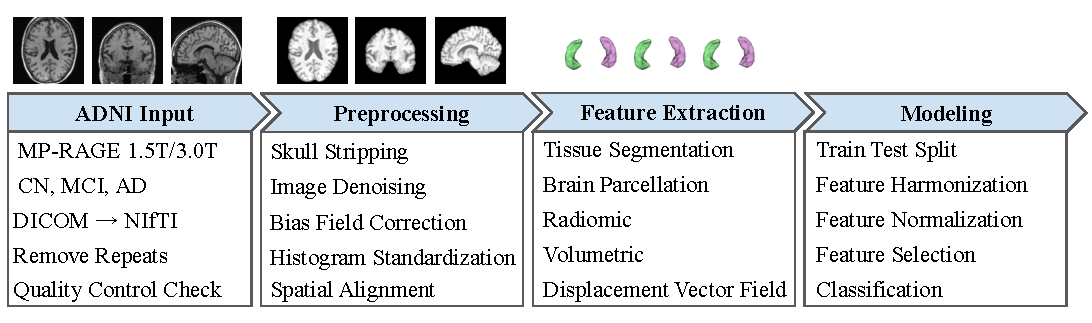
\includegraphics[width=1.0\textwidth]{graphics/diagrama.pdf} % Substitua pelo nome do seu arquivo
	\caption{Diagrama esquemático do pipeline de processamento e análise radiômica.}
	\label{fig:pipeline}
\end{figure}

Na etapa de pré processamento, todas as imagens foram processados por meio de uma cadeia sequencial de passos, composta pelas seguintes etapas:

\textbf{Extração de crânio (\emph{Skull stripping}):} Executada utilizando um modelo de extração encefálica baseado em aprendizagem profunda, treinado em imagens T1 e disponível na biblioteca ANTsPyNet (\code{antspynet.brain\_extraction}, \code{modality="t1"}) \cite{tustison-2021}.

\textbf{Filtragem de ruído (\emph{Denoising}):} Aplicação de um filtro de médias não locais adaptativas otimizado para ruído ricianiano \cite{manjon-2010}, implementado através da função \code{ants.denoise\_image}. Foram adotados os parâmetros \code{noise\_model="Rician"}, raio de \emph{patch} $p=2$, raio de busca $r=3$ e \code{mask=None}. O parâmetro \code{shrink\_factor=1}, específico do pacote ANTs, foi utilizado para desativar a subamostragem (\emph{downsampling}) interna, constituindo uma diretriz de implementação da ferramenta e não uma modificação da formulação matemática original.

\textbf{Correção de campo de viés (\emph{Bias field correction}):} Aplicação do algoritmo N4ITK \cite{tustison-2010} por meio da função \code{ants.n4\_bias\_field\_correction}, configurado com \code{shrink\_factor=3}, \code{convergence=\{iters: [50, 50, 50, 50], tol: }\(1\times10^{-7}\)\code{\}} (representando quatro níveis de multirresolução), \code{spline\_param=200}, \code{rescale\_intensities=True} e \code{mask=None}.

\textbf{Normalização de intensidade (\emph{Histogram matching}):} As intensidades dos volumes T1 foram padronizadas utilizando a técnica de pareamento de histograma (\emph{histogram matching}) \cite{nyul-2000} em relação ao \emph{template} fixo MNI152 2009c \cite{fonov-2011}. Esta etapa foi implementada com a função \code{ants.histogram\_match\_image2} (\code{transform\_domain\_size=128}, \code{match\_points=16}), aplicada após uma normalização \code{min-max} conduzida de forma independente para as imagens fonte e de referência. As máscaras encefálicas, tanto da imagem original quanto da referência, foram estimadas via \code{ants.get\_mask}. As intensidades pareadas foram subsequentemente reescalonadas com base no percentil 99,9 dos voxels pertencentes à região encefálica da imagem de referência. É crucial notar que este procedimento foi executado independentemente \textbf{por imagem}, sem a estimação de parâmetros de intensidade em nível de coorte. Embora o \emph{histogram matching} atenue distorções macroscópicas de escala de cinza, ele não modela efeitos de lote (\emph{batch effects}) inerentes a diferentes \emph{scanners} ou fabricantes ao nível dos atributos texturais. Para mitigar potenciais vieses multicêntricos, a harmonização via NeuroComBat aplicada de forma particionada por \emph{fold} de validação cruzada \cite{fortin-2018} foi conduzida como uma análise de sensibilidade opcional.

\textbf{Parcelamento anatômico e segmentação tecidual:} Os mapas de regiões de interesse (ROI) foram gerados utilizando a função \code{antspynet.desikan\_killiany\_tourville\_labeling} \cite{tustison-2021} (\code{modality="t1"}, \code{do\_preprocessing=True}), com ênfase na identificação dos hipocampos (rótulos DKT 17 e 53) e demais regiões empregadas na extração radiômica. Adicionalmente, a segmentação volumétrica em Líquido Cefalorraquidiano (CSF), Substância Cinzenta (GM) e Substância Branca (WM) — correspondentes aos rótulos 1, 2 e 3 — foi realizada via \code{antspynet.deep\_atropos}, mantendo a mesma configuração de modalidade e pré-processamento. Esta decisão metodológica visou assegurar a compatibilidade das imagens de entrada com a distribuição de dados na qual os pesos dos modelos de aprendizagem profunda do ANTsPyNet foram otimizados, ainda que isso implicasse certa redundância procedimental nas normalizações de intensidade e espaço. Ressalta-se, contudo, que os mapas de rótulos resultantes foram utilizados exclusivamente para a delineação de ROIs e cômputo de frações teciduais, e que as transformações geométricas e de intensidade subjacentes ao ANTsPyNet não figuraram como estágios treináveis no modelo preditivo final.

\textbf{Interpolação isotrópica e Alinhamento espacial:} Para satisfazer os requisitos de extração de atributos radiômicos, os volumes T1 já pré-processados foram submetidos a um registro puramente \textbf{rígido} (6 graus de liberdade: translação e rotação, sem componentes afins ou deformáveis) em relação ao \emph{template} MNI152 2009c, estabelecendo uma grade isotrópica com resolução de \(1{,}0\)\,mm. Neste contexto, o \emph{template} atuou estritamente como um referencial geométrico (espaçamento e orientação canônicos), não como um alvo para normalização anatômica não-linear. O cômputo da transformação e a subsequente interpolação da imagem T1 foram realizados via \code{ants.registration} (\code{type\_of\_transform="Rigid"}, interpolador \code{"linear"}), definindo o \emph{template} MNI como imagem fixa e a T1 do paciente como imagem móvel. A matriz de transformação resultante (\code{fwdtransforms}) foi então aplicada aos mapas de parcelamento DKT originais, segmentações de classes teciduais e máscara encefálica  através da função \code{ants.apply\_transforms}. Para essa etapa, a imagem T1 reamostrada serviu como referência espacial, utilizando-se mandatoriamente o interpolador de vizinho mais próximo (\code{"nearestNeighbor"}) para preservar a integridade dos identificadores inteiros das classes anatômicas. Consequentemente, a imagem de intensidade e suas respectivas máscaras alinham-se perfeitamente na mesma pose, grade e orientação, preservando a morfologia original do sujeito sujeita apenas a uma isometria e a uma única operação de interpolação. Por esta razão, o parâmetro \code{resampledPixelSpacing} foi deliberadamente omitido durante a configuração da biblioteca PyRadiomics, evitando uma segunda (e deletéria) interpolação espacial prévia à extração das matrizes de textura.

\textbf{Discretização de intensidade (\emph{Binning}):} Em consonância com as diretrizes da IBSI, as imagens foram discretizadas antes do cálculo das matrizes de textura. Empregou-se a estratégia de discretização por Número Fixo de \emph{Bins} (FBN) computada de forma independente por ROI, fixando-se a contagem em 64 \emph{bins} (\code{binCount=64}). Como as imagens já haviam sido normalizadas previamente na etapa de \emph{histogram matching}, a opção de normalização interna por z-score da biblioteca PyRadiomics foi mantida desativada (\code{normalize=False}), operando-se diretamente sobre as intensidades pareadas.
	
\subsection{Extração de atributos}\label{sec:feature-extraction}

Por aquisição extraem-se cinco famílias: volume, forma, textura GLCM, primeira ordem e deslocamento normativo.
O armazém guarda o bloco IBSI completo e os mapas do DVF.
O classificador recebe a \emph{classe} de cada família após uma denylist só de definição (\code{keep\_*\_feat} em \code{ablation\_prep.py}; Tabela~\ref{tab:dims}): não há lista permitida de 4--5 nomes.
A selecção amostral (variância, correlação, pool \code{l1\_stable}) corre depois, só no treino externo. \sugestao{}{Todas as definições dos atributos radiomicos são fornecidas no Image Biomarker Standardization Initiative (IBSI) reference manual \url{https://ibsi.readthedocs.io/en/latest/} ONLINE**}

\subsubsection{Atributos volumétricos}\label{subsubsec:feat_vol}

Por ROI intersectada com a máscara encefálica, \code{3\_feat\_vol.py} regista volumes em mm$^3$ e fracções \emph{dentro da ROI}: $\mathtt{gm\_norm}=V_{\mathrm{GM}}/V_{\mathrm{ROI}}$ (análogo para WM e LCR).
O ICV (\code{ICV\_mask\_mm3}) é o volume da máscara encefálica (linha \code{\_\_global\_\_}).
No pós-processamento aplica-se homotetia de volume: comprimentos$/\,\mathrm{ICV}^{1/3}$, áreas$/\,\mathrm{ICV}^{2/3}$, volumes$/\,\mathrm{ICV}$; \code{SurfaceVolumeRatio} (já $A/V$) multiplica-se por $\mathrm{ICV}^{1/3}$. As fracções teciduais \textbf{não} se renormalizam pelo ICV --- não são volumetria clássica em mm$^3$ \cite{wyman-2013}.
Entram \code{gm\_norm}, \code{wm\_norm}, \code{csf\_norm} e \code{original\_shape\_MeshVolume} (já $/\mathrm{ICV}$).
Saem volumes crus em mm$^3$.
O volume de malha fica no bloco de volume, não no de forma.

\subsubsection{Atributos radiómicos (PyRadiomics)}\label{subsubsec:radiomics}

Forma, textura e primeira ordem extraem-se com PyRadiomics \code{3.1.1.dev111+g8ed579383} \cite{griethuysen-2017}.
Nomes e definições seguem a terminologia IBSI da biblioteca \cite{zwanenburg-2020}; não se reivindica validação IBSI independente.

A extração é independente por ROI e aquisição (\code{3\_feat\_rad.py}), sobre volumes T1 já registados rigidamente ao MNI152 2009c em grelha isotrópica de $1{,}0$\,mm (interpolação linear na imagem; vizinho mais próximo nas máscaras).
O PyRadiomics não reamostra (\code{resampledPixelSpacing} omitido), evitando segunda interpolação.
Grelha e afinidade imagem/máscara verificam-se com tolerância absoluta \(10^{-5}\).
Cada rótulo anatómico intersecta a máscara encefálica; ROI ausente grava-se NaN.
Só o tipo de imagem \code{Original} (sem LoG nem wavelet).
Discretização por contagem fixa de bins (\code{binCount}$=64$; \code{binWidth} omitido), adequada a unidades MRI arbitrárias e para evitar o default CT \code{binWidth}$=25$.
Controlos restantes nos defaults da biblioteca (\code{normalize=False}, \code{force2D=False}, \code{distances=[1]}, \code{symmetricalGLCM=True}).

Por ROI e visita o \textbf{armazém} guarda 107 descritores: 18 de primeira ordem, 14 de forma, 24 GLCM, 16 GLRLM, 16 GLSZM, 5 NGTDM e 14 GLDM.
Nas ablações hipocampais oficiais, após denylist só de definição (\code{ablation\_prep.py}), entram três subcategorias radiómicas (Tabela~\ref{tab:pyradiomics-features}):

\begin{itemize}
	\item \textbf{primeira ordem:} 16 \code{original\_firstorder\_*} excepto \code{Energy} e \code{TotalEnergy} (escalam com o número de voxels);
	
	\item \textbf{forma:} 12 \code{original\_shape\_*} excepto \code{MeshVolume} e \code{VoxelVolume} (tamanho fica no bloco volumétrico; \code{MeshVolume} entra já $/\mathrm{ICV}$; eixos/diâmetros e área já homotéticos);
	
	\item \textbf{textura:} os 24 \code{original\_glcm\_*} (GLCM Original); saem GLRLM, GLSZM, GLDM, NGTDM e filtros wavelet/LoG.
\end{itemize}

Cada sufixo conta $\times$ L e R; em \code{t1\_only} $\times 1$ visita e em Q4 (\code{t1\_d21\_d32}) $\times 3$ slots.
Contagens L$+$R \emph{antes} do L1: Tabela~\ref{tab:dims}.

\begin{table}[htbp]
	\centering
	\caption{Atributos PyRadiomics retidos nas ablações hipocampais (após denylist). Prefixo \code{original\_} omitido na coluna de nomes para legibilidade; no CSV o nome completo inclui \code{original\_firstorder\_}, \code{original\_shape\_} ou \code{original\_glcm\_}.}
	\label{tab:pyradiomics-features}
	\small
	\begin{tabular}{@{}llp{0.62\textwidth}@{}}
		\toprule
		Subcategoria & $n$ & Atributos (sufixo) \\
		\midrule
		Primeira ordem
		& 16
		& \code{10Percentile}, \code{90Percentile}, \code{Entropy}, \code{InterquartileRange},
		\code{Kurtosis}, \code{Maximum}, \code{Mean}, \code{MeanAbsoluteDeviation},
		\code{Median}, \code{Minimum}, \code{Range}, \code{RobustMeanAbsoluteDeviation},
		\code{RootMeanSquared}, \code{Skewness}, \code{Uniformity}, \code{Variance} \\
		\addlinespace
		Forma
		& 12
		& \code{SurfaceArea}, \code{SurfaceVolumeRatio}, \code{Sphericity}, \code{Elongation},
		\code{Flatness}, \code{LeastAxisLength}, \code{MajorAxisLength}, \code{MinorAxisLength},
		\code{Maximum2DDiameterColumn}, \code{Maximum2DDiameterRow},
		\code{Maximum2DDiameterSlice}, \code{Maximum3DDiameter} \\
		\addlinespace
		Textura (GLCM)
		& 24
		& \code{Autocorrelation}, \code{ClusterProminence}, \code{ClusterShade},
		\code{ClusterTendency}, \code{Contrast}, \code{Correlation},
		\code{DifferenceAverage}, \code{DifferenceEntropy}, \code{DifferenceVariance},
		\code{Id}, \code{Idm}, \code{Idmn}, \code{Idn}, \code{Imc1}, \code{Imc2},
		\code{InverseVariance}, \code{JointAverage}, \code{JointEnergy},
		\code{JointEntropy}, \code{MCC}, \code{MaximumProbability},
		\code{SumAverage}, \code{SumEntropy}, \code{SumSquares} \\
		\midrule
		Total
		& 52
		& --- \\
		\bottomrule
	\end{tabular}
\end{table}

\subsubsection{Atributos de deslocamento}\label{sec:displacement-features}

A referência é o atlas groupwise CN do sexo e da década em $i_1$, independente do diagnóstico \cite{wyman-2013}, e mantém-se em $i_2$ e $i_3$.
Em cada visita, SyN com template CN \textbf{fixo} e T1 clínico \textbf{móvel} (\code{3\_feat\_gen\_dvf\_v2.py}).
Os mapas vivem no domínio do template. O campo obtém-se aplicando $I_t=[\text{affine},\text{inverse warp}]$ às coordenadas físicas do template (fixed $\rightarrow$ moving):

\begin{equation}
	\mathbf{u}_t(x)=I_t(x)-x,\qquad x\in\Omega_{\mathrm{CN}}.
	\label{eq:dvf-template}
\end{equation}

ROIs e máscara encefálica do sujeito transportam-se ao template pela cadeia directa (Warp$+$Affine, vizinho mais próximo).
De $\mathbf{u}_t$ derivam-se $\log J$, $\|\mathbf{u}\|$, divergência, $(u_x,u_y,u_z)$, rotacional, escalares de Green--Lagrange e $\|\varepsilon\|_F$ da deformação infinitesimal $\varepsilon=\tfrac12(H+H^{\top})$ \cite{bouke-2023}.
Não há mapas $i_a\rightarrow T_b$: $i_2$ e $i_3$ são desvio ao mesmo âncora CN, não deformação inter-visita.
Por ROI hipocampal no template agregam-se média, desvio-padrão, percentis e, para $\log J$, $\|\mathbf{u}\|$ e $\|\varepsilon\|_F$, variância, assimetria e curtose.

Entram momentos de \code{mag\_}, \code{logjac\_} e \code{strain\_fro\_} (15 sufixos por lado na representação longa).
Saem componentes \code{ux}/\code{uy}/\code{uz}, sufixos \code{\_n} e percentis.
\code{strain\_fro\_mean} resume a norma de Frobenius de Green--Lagrange; \code{strain\_fro\_variance} a da $\varepsilon$ infinitesimal --- tensores distintos.

A extração de atributos foi realizada de forma independente para cada aquisição sobre um conjunto fixo de 20 regiões de interesse (ROIs) bilaterais definidas pelo atlas Desikan-Killiany-Tourville (DKT) (hipocampo, amígdala, tálamo, núcleo accumbens, ventrículo lateral inferior, cíngulo posterior, istmo do cíngulo, cíngulo anterior rostral, orbitofrontal medial e ínsula). Cada ROI foi previamente intersectada com a máscara encefálica do sujeito; em casos excepcionais de regiões anatomicamente ausentes na segmentação de um determinado sujeito, os atributos foram computados como nulos (NaN). Extraíram-se cinco famílias de atributos quantitativos (volumetria, forma, textura, estatísticas de primeira ordem e tensores de deslocamento normativo), divididos em dois domínios espaciais de cômputo: os cálculos morfológicos, texturais e densitométricos ocorreram no espaço anatômico do sujeito rigidamente alinhado (grelha isotrópica de $1{,}0$\,mm do MNI), enquanto o campo de deslocamento vetorial foi construído no domínio de referência do template \emph{groupwise}. Após o armazenamento abrangente, aplicou-se uma lista de exclusão fixa (\emph{denylist}) para restringir os dados fornecidos ao classificador.

\textbf{Volumetria.} As matrizes de classes teciduais (LCR, Substância Cinzenta e Substância Branca) e a máscara encefálica foram avaliadas na mesma grelha espacial, calculando-se os volumes locais pelo produto das dimensões (\emph{zooms}) dos \emph{voxels}. Foram extraídos os volumes absolutos por ROI e, crucialmente, as frações volumétricas teciduais \textbf{dentro da própria ROI} (ex: $V_{\text{GM}}/V_{\text{ROI}}$). O volume intracraniano total (ICV) foi estimado como o volume absoluto da máscara encefálica total e armazenado em uma linha de controle (\code{\_\_global\_\_}). Como etapa de normalização morfológica por homotetia, comprimentos (eixos e diâmetros PyRadiomics) dividem-se por \(\mathrm{ICV}^{1/3}\), áreas de superfície por \(\mathrm{ICV}^{2/3}\) e volumes absolutos (mm$^3$ e \code{MeshVolume}) por \(\mathrm{ICV}\); \code{SurfaceVolumeRatio} multiplica-se por \(\mathrm{ICV}^{1/3}\). As frações teciduais intrarregionais \textbf{não} sofreram renormalização adicional. Das características armazenadas, o modelo consumiu apenas as proporções teciduais (\code{gm\_norm}, \code{wm\_norm}, \code{csf\_norm}) e o volume total da malha (\code{original\_shape\_MeshVolume} já $/\mathrm{ICV}$).

\textbf{Radiômica e Textura.} A extração de morfometria e atributos baseados nas intensidades originais (não-filtradas) procedeu com o ecossistema \emph{PyRadiomics} (\code{v.3.1.1.dev111}), utilizando definições nomenclaturais da \emph{Image Biomarker Standardisation Initiative} (IBSI). Para assegurar a invariância direcional da matriz 3D, a textura foi avaliada com os parâmetros \code{force2D=False}, \code{distances=[1]} e \code{symmetricalGLCM=True}. Devido à etapa prévia de reamostragem rígida isotrópica no pacote ANTsX (garantindo equivalência das transformações afins entre imagem e máscara até uma tolerância atol $10^{-5}$), o parâmetro de reamostragem interna da biblioteca (\code{resampledPixelSpacing}) foi omitido, e a normalização baseada em escore-z permaneceu desativada (\code{normalize=False}), operando sobre a intensidade global pareada pelo \emph{histogram matching}. A discretização de intensidades obedeceu à premissa do Número Fixo de Bins (FBN), fixando \code{binCount=64} localmente por ROI e forçando a omissão do tamanho estático do \emph{bin} (\code{binWidth}). Antes da filtragem para classificação (\emph{denylist}), o cômputo completo gerou 107 descritores por ROI por visita (18 de primeira ordem, 14 de forma, 24 GLCM, e 51 matrizes de textura não-estruturais NGTDM, GLSZM, GLRLM, GLDM). O pipeline final alimentou os estimadores com os seguintes subconjuntos independentes:

\begin{itemize}
	\item \textbf{Forma (\emph{Shape}):} 12 parâmetros IBSI de morfologia em três dimensões (ex: esfericidade, achatamento, eixos), excluindo-se as medidas brutas de \code{MeshVolume} e \code{VoxelVolume}.
	\item \textbf{Estatísticas de Primeira Ordem (\emph{First-order}):} 16 estimativas de distribuição, dispersão e medidas centrais derivadas do histograma global de cada ROI, com exclusão de métricas brutas somatórias (\code{Energy} e \code{TotalEnergy}).
	\item \textbf{Textura:} 24 distribuições da \emph{Gray Level Co-occurrence Matrix} (GLCM), descartando-se todas as demais matrizes avançadas.
\end{itemize}

\subsection{Deslocamento normativo (\emph{displacement}).}
Para quantificar o desvio biomecânico local (atrofia ou expansão) relativamente a um referencial de envelhecimento saudável, registou-se cada imagem clínica, já alinhado rigidamente a 1\,mm, a um \emph{template groupwise} CN estratificado por sexo biológico e década de idade. No SyN não linear~\cite{avants-2011a}, o \emph{template} CN foi a imagem \textbf{fixa} e imagem clínica a imagem \textbf{móvel}, com interpolação B-spline. O diagnóstico não entra na escolha do atlas: o mesmo \emph{template}, definido pelo sexo e pela década da visita \emph{baseline} ($i_1$), aplica-se a imagens $i_1$, $i_2$ e $i_3$. Cada exame é registado de forma independente a esse referencial estacionário; não há cadeia de \emph{warps} entre visitas.

O campo de deslocamento foi avaliado no \textbf{domínio do template}. A transformação inversa $I_t$ (fixa $\to$ móvel, i.e., template $\to$ sujeito), composta pelo afim e pelo \emph{inverse warp}, mapeia coordenadas físicas $x\in\Omega_{\mathrm{CN}}$ para o espaço clínico. O deslocamento é definido por
\[
\mathbf{u}_t(x)=I_t(x)-x.
\]
As máscaras DKT e a máscara encefálica do sujeito foram transportadas para $\Omega_{\mathrm{CN}}$ pela transformação \textbf{directa} (móvel $\to$ fixa: \emph{warp} + afim), utilizando o interpolador de vizinho mais próximo.

A partir de $\mathbf{u}_t$ derivaram-se o logaritmo do jacobiano (\code{logjac}), a magnitude do deslocamento (\code{mag}) e a norma de Frobenius do tensor de deformação infinitesimal $\varepsilon=\tfrac12(H+H^{\top})$, onde $H=\nabla\mathbf{u}$ (\code{strain\_fro}). O classificador reteve, por ROI e por mapa, cinco estatísticas transversais: média, desvio-padrão, variância amostral, assimetria de Fisher e curtose. Percentis ($p_{05}$, $p_{50}$, $p_{95}$), contagem de voxels e componentes direcionais ($u_x$, $u_y$, $u_z$), bem como divergência e rotacional, foram excluídos do modelo preditivo. Especificamente em \code{strain\_fro}, a média e o desvio-padrão correspondem ao tensor de Green--Lagrange por motivos de compatibilidade com versões prévias do sistema extraído; enquanto variância, assimetria e curtose utilizam rigorosamente a métrica $\lVert\varepsilon\rVert_F$ do campo infinitesimal.

\subsection{Construção de \emph{templates groupwise} estratificados}\label{sec:groupwise}

Para reduzir o viés inerente à utilização de um único sujeito de referência~\cite{reuter-2012} e fornecer um espaço normativo demografamente adequado, construíram-se \emph{templates} volumétricos médios a partir de imagens T1 pré-processadas exclusivas de indivíduos cognitivamente normais (CN). Os \emph{templates} foram estratificados por sexo e década de idade ($50$--$59{,}9$, $60$--$69{,}9$, $\ldots$, $90$--$99{,}9$ anos; idades $<50$ e $>99{,}9$ foram atribuídas aos estratos extremos), servindo de referência de envelhecimento saudável para o registro deformável visita a visita.

Por estrato sexo--década reteve-se até $N_{\max}=20$ aquisições CN. Acima desse limite, aplicou-se amostragem aleatória sem reposição garantida por semente fixa (\code{RANDOM\_SEED=7}). A amostra CN foi fixada uma única vez, antes da validação cruzada aninhada, assegurando a não reamostragem nos \emph{folds} externos. Nenhum participante pertencente às classes sMCI ou pMCI contribuiu para a confecção dos \emph{templates}. Consequentemente, para o desfecho primário sMCI vs pMCI, os atlas atuam como referências normativas estritas disjuntas das duas classes prognósticas, descartando-se qualquer dependência transformacional ajustada por \emph{fold}.

O alinhamento \emph{groupwise} foi inicializado com um pré-registro global mascarado (transformações rígidas seguidas de afins) a um referencial alvo comum. O \emph{template} inicial $T^{(0)}$ foi estabelecido como a média aritmética das imagens pré-alinhadas no espaço do alvo. Seguiu-se refinamento não linear via algoritmo SyN~\cite{avants-2014} ao longo de cinco iterações: em cada ciclo, todas as imagens do estrato foram registradas não linearmente ao \emph{template} corrente sob máscara encefálica, e este atualizou-se iterativamente pela média global das imagens deformadas. Após a última iteração, recomputou-se a máscara encefálica no \emph{template} médio e as intensidades intracranianas sofreram reescalonamento fotométrico (recorte restrito aos percentis 2 e 98 com mapeamento linear exato para $[0,1]$). Este passo harmoniza visualmente o contraste inter-estratos sem corromper as transformações deformáveis alocadas ao pipeline prognóstico.

\subsection{Registro normativo visita a visita}\label{subsec:deslocamento_longitudinal}

Os atributos de deformação biomecânica derivam estritamente de um registro normativo transversal computado visita a visita, abstendo-se da formulação de campos de diferença diretos inter-visitas. Para cada participante, o \emph{template} CN designado foi fixado com base no sexo e na década biológica correspondentes exclusivamente à primeira visita de entrada no modelo ($i_1$), independentemente de seu diagnóstico clínico corrente~\cite{wyman-2013}. Esta atribuição normativa ancorada persistiu inalterada durante as modelagens das visitas subsequentes ($i_2$ e $i_3$).

Em cada instante avaliativo $t\in\{T_1,T_2,T_3\}$, executou-se um procedimento SyN espacialmente independente na grelha isotrópica de $1{,}0$\,mm: determinando o \emph{template} CN como imagem \textbf{fixa} e a aquisição T1 clínica pré-processada como imagem \textbf{móvel} (\code{ants.registration}). O otimizador estimou a transformação clínico$\to$\emph{template} $F_t$ (móvel $\to$ fixa) e sua contraparte espacial inversa $I_t$ (fixa $\to$ móvel). Matrizes afins, \emph{warps} diretos e inversos foram registrados isoladamente por aquisição.

A informação longitudinal foi incorporada ao classificador preditivo através da representação sistêmica "Q4": para cada descritor estatístico regional (ROI) extraído do registro transversal, procedeu-se com a concatenação estrita do nível basal com as duas sucessivas variações discretas temporais $\{\mathrm{feat}_{T_1},\,\Delta_{21},\,\Delta_{32}\}$, formalizadas como $\Delta_{21}=\mathrm{feat}_{T_2}-\mathrm{feat}_{T_1}$ e $\Delta_{32}=\mathrm{feat}_{T_3}-\mathrm{feat}_{T_2}$. Reitera-se enfaticamente que \textbf{não} ocorreu composição sintética espacial de \emph{warps} cruzando os eixos de visita (e.g., $I_{T_2}\circ F_{T_1}$) e \textbf{não} ocorreu cálculo parametrizado de campos transicionais \emph{baseline}$\to$\emph{follow-up}. Cada instância de visita mensurou o desvio anatômico absoluto contra a mesma referência CN comum estacionária; resultando em uma trajetória temporal modelada exclusivamente sob o domínio dos momentos escalares extraídos nas ROIs, não através de um mapeamento \emph{warp} intra-sujeito explícito.

\subsection{Desenho experimental}\label{sec:experiments}

O desfecho primário avaliado é a classificação binária entre sMCI e pMCI, estratificada em um arranjo fatorial constituído por quatro coortes independentes, delineadas pela combinação da janela clínica preditiva e da frequência de intervalo entre as aquisições (Tabela~\ref{tab:coortes}): \code{36m\_6m} ($125/106$), \code{36m\_12m} ($121/33$), \code{48m\_6m} ($73/120$) e \code{48m\_12m} ($72/48$). A inclusão em qualquer coorte exigiu rigorosamente a disponibilidade de três exames de RM T1 consecutivos portando parcelamento hipocampal bilateral identificável nos instantes $i_1$, $i_2$ e $i_3$, com intervalos inter-visitas limitados a uma tolerância estrita de $\pm 2$ meses.

A restrição do tamanho amostral global ($n$) reflete as balizas metodológicas exigidas para a modelagem: a necessidade de três vetores preditivos completos e sequenciais, bem como a observância estrita do comportamento clínico temporal. Com o intuito de apoiar a capacidade de generalização do modelo e mitigar o risco de vazamento de dados, o particionamento ocorreu de forma restrita em nível de paciente (\emph{patient-level split}). Assim, todos os três pontos temporais de um mesmo indivíduo foram alocados ao mesmo estrato, assegurando a independência adequada entre os conjuntos de treinamento e teste.

A caracterização demográfica, o delineamento metodológico e as análises principais --- que abrangem as ablações de arquitetura clínica (\code{leaky ablation}), a identificação interpretável de atributos selecionados e a diferenciação de referências (CN vs. AD) --- foram ancorados na coorte principal do estudo, a \code{48m\_12m} ($n=120$). Em contrapartida, as demais matrizes (\code{36m\_6m}, \code{36m\_12m} e \code{48m\_6m}) compuseram as análises de sensibilidade, permitindo avaliar a consistência dos achados sob diferentes janelas clínicas e intervalos de aquisição. Adicionalmente, o delineamento multimodal via fusão tardia (\emph{late fusion}), sob três especificações arquiteturais distintas, operou sistematicamente perpassando o espectro das quatro coortes.

\textbf{Prevenção de Vazamento de Dados.} Para obter estimativas de validação cruzada robustas e minimizar o risco de fuga de informação (\emph{data leakage}), estabeleceu-se uma distinção clara entre os processos \emph{fixos por imagem} e os métodos \emph{dependentes da amostra}. Procedimentos intrínsecos ao processamento das imagens --- incluindo normalização craniana, \emph{denoising}, parcelamento atlas-guiado, registro normativo e extração radiômica --- foram executados uma única vez por volume. Sob configurações pré-definidas e algoritmos fixos, essas etapas operaram independentemente da existência dos rótulos de classe (sMCI/pMCI) e não requereram calibrações baseadas no agrupamento da população. Da mesma forma, os limites de controle de qualidade (QC) e a construção dos \emph{templates} normativos CN foram definidos integralmente antes da fase de seleção do classificador.

Por outro lado, as transformações matemáticas baseadas na configuração e na distribuição estatística dos dados foram restritas à malha interna da validação cruzada aninhada (\emph{nested cross-validation}). Filtros de covariância cruzada colinear, normalização por \emph{z-score}, regularização linear, parametrização estocástica e a definição dos limiares de decisão de Youden foram calibrados apenas com os dados dos estratos de treinamento. Uma vez ajustados, esses coeficientes foram aplicados aos \emph{folds} externos de teste, mantendo a integridade e a validade da avaliação preditiva.

\subsubsection{Métricas de avaliação}
\label{subsubsec:evaluation-metrics}

Seja $s_{ir} = \widehat{\Pr}(y=1 \mid x_i)$ a probabilidade \emph{Out-Of-Fold} (OOF) predita para o participante $i$ na repetição $r \in \{1,\ldots,R\}$ (com $R=10$). Este valor é obtido através da concatenação das partições (\emph{folds}) de teste dos cinco estratos externos disjuntos em cada repetição. Todos os classificadores avaliados produziram probabilidades estritas (\code{predict\_proba}), sendo aplicada a calibração de Platt (\code{probability=True}) aos modelos SVM. 

O estimador primário de desempenho do modelo estabelece-se pela média das probabilidades calibradas de cada paciente ao longo das $R$ repetições:
\begin{equation}
	\bar{s}_i = \frac{1}{R}\sum_{r=1}^{R}s_{ir}.
	\label{eq:prob-mean}
\end{equation}
A métrica primária é a Área Sob a Curva ROC ao nível do paciente ($\mathrm{AUC}_{\mathrm{patient}}$), calculada sobre essas probabilidades agregadas por intermédio da estatística de Mann-Whitney. Definindo $n_+$ e $n_-$ como o número de amostras positivas e negativas, e assumindo o tratamento de empates com peso de $1/2$, o estimador primário consolida-se como:
\begin{equation}
	\mathrm{AUC}_{\mathrm{patient}}
	\equiv
	\widehat{\mathrm{AUC}}_{\mathrm{agg}}
	= \mathrm{AUC}\!\left(\{(y_i,\bar{s}_i)\}_{i=1}^{n}\right)
	= \frac{1}{n_+ n_-}
	\sum_{i:\,y_i=1} \sum_{j:\,y_j=0}
	\left(
	\mathbb{I}(\bar{s}_i > \bar{s}_j)
	+ \tfrac{1}{2}\,\mathbb{I}(\bar{s}_i = \bar{s}_j)
	\right),
	\label{eq:auc-pooled}
\end{equation}
em que $\mathbb{I}(\cdot)$ representa a função indicadora. 

Este estimador distingue-se metodologicamente de outros três resumos reportados nas análises: (i) a AUC individual de cada \emph{fold}, cuja média e desvio-padrão (DP) nas 50 avaliações descrevem a variabilidade entre os modelos treinados, e não a incerteza amostral da $\widehat{\mathrm{AUC}}_{\mathrm{agg}}$; (ii) a média das AUCs por repetição ($\overline{\mathrm{AUC}}$); e (iii) a AUC do tipo \emph{pooled}, que atua como resumo de sensibilidade ao concatenar os $R$ registros por participante antes do cálculo da área, sem os mediar. Adicionalmente, os desvios-padrão tabelados para o estimador primário, bem como os intervalos de confiança de 95\% e os testes de hipótese para a variação de desempenho ($\Delta\mathrm{AUC}$), foram obtidos estritamente por \emph{bootstrap} pareado (com $B \in \{2000, 5000\}$ reamostragens) operando sobre os escores agregados $\{\bar{s}_i\}$.

Para as métricas dependentes de limiar, o ponto de operação ótimo $\tau^*$ foi determinado maximizando-se o índice de Youden sobre os escores OOF do treinamento externo (gerados pela validação cruzada interna):
\begin{equation}
	J(\tau) = \mathrm{TPR}(\tau) + \mathrm{TNR}(\tau) - 1,
	\qquad
	\tau^{*} = \arg\max_{\tau \in [0,1]} J(\tau),
	\label{eq:youden}
\end{equation}
em que $\mathrm{TPR}$ e $\mathrm{TNR}$ representam as taxas de verdadeiros positivos e verdadeiros negativos, respectivamente. A busca por $\tau^*$ restringiu-se ao domínio probabilístico $[0,1]$, descartando-se limiares oriundos de escores brutos de decisão (\code{decision\_function}). Um limiar distinto foi ajustado para cada \emph{fold} externo e aplicado exclusivamente ao seu conjunto de teste correspondente. Desse modo, métricas como acurácia, sensibilidade, especificidade e pontuação F1 (\emph{F1-score}) foram computadas de forma isolada por \emph{fold} e consolidadas como média $\pm$ DP. Em nenhum momento procedeu-se à reestimação de um limiar global sobre predições misturadas de \emph{folds} distintos.

\textbf{Constantes analíticas e hiperparâmetros.} A fim de garantir a reprodutibilidade, fixou-se a semente aleatória inicial em 42, com derivações determinísticas para repetições e \emph{folds} aninhados. Estabeleceram-se $k_{\mathrm{out}}=k_{\mathrm{in}}=5$ partições. O pré-processamento estático incluiu um filtro de variância para feições constantes (variância $<0{,}01$) e um filtro de colinearidade iterativo de Pearson ($|\rho|>0{,}85$), configurado para não suprimir mutuamente feições temporais (T1, D21, D32) derivadas de uma mesma região anatômica. A seleção de atributos por estabilidade baseou-se em penalização $\ell_1$ ($C=0{,}1$) através de $B=50$ réplicas de \emph{bootstrap}, impondo-se uma frequência mínima de retenção $\pi=70\,\%$ por grupo anatômico e \code{stable-pool-min-timepoints=0}. Por fim, a sintonia de hiperparâmetros foi orquestrada pelo algoritmo estimador de Parzen (Optuna TPE, com \code{optuna-trials=10}), preterindo-se abordagens tradicionais de busca exaustiva em grade.

\subsubsection{Classificação e Inferência Estatística}

\textbf{Modelo Classificador Primário.} O estimador primário estabelecido para a totalidade das análises foi a Máquina de Vetores de Suporte (SVM) \cite{cortes-1995}, configurada com núcleo linear ou de base radial (RBF). O escopo deste estudo avalia fundamentalmente a capacidade preditiva da representação temporal de biomarcadores (família matemática $\times$ codificação longitudinal $\times$ fusão), preterindo o \emph{benchmarking} de arquiteturas de aprendizado de máquina. A fixação estrita da SVM isola os contrastes experimentais de vieses algorítmicos inerentes à variação de capacidade do modelo e aos métodos intrínsecos de regularização, além de figurar como padrão consolidado em estudos de discriminação morfológica na base ADNI sob a condição de alta dimensionalidade de atributos em amostras restritas ($p \approx n$) \cite{cuingnet-2011}. Métodos adicionais, como Florestas Aleatórias (\emph{Random Forest}) \cite{breiman-2001} e regressão logística com regularização \emph{Elastic-Net} \cite{zou-2005}, foram relegados a análises de sensibilidade secundárias, não compondo as tabelas oficiais do desfecho primário. Ressalta-se que a etapa de seleção de atributos (\code{l1\_stable}) operou sempre a montante da SVM, desconectando o rastreio esparso da regra de decisão final.

\textbf{Calibração e Sintonia.} A otimização hiperparamétrica da SVM foi conduzida exclusivamente sobre a validação cruzada interna, maximizando a AUC média local através da árvore de estimadores de Parzen (algoritmo Optuna TPE, orquestrado para 10 iterações de busca), em detrimento da tradicional e exaustiva busca em grade (\emph{grid search}). O domínio de busca englobou a escolha do núcleo (Linear vs. RBF), o parâmetro de penalização $C \in [10^{-2}, 10]$ (em escala logarítmica), e os pesos de classe (\code{class\_weight} $\in \{\mathrm{None}, \mathrm{balanced}\}$), com limite de iterações do \emph{solver} fixado em 2000. Para obtenção de métricas probabilísticas contínuas, ajustou-se a SVM com o parâmetro \code{probability=True}, convertendo os valores nominais de decisão em probabilidades limpas (\code{predict\_proba}) mediante escalonamento logístico de Platt interno ao estimador. Esta calibração probabilística reajustou-se a cada iteração do treinamento, blindada contra qualquer contaminação proveniente dos subconjuntos de teste externo.

\textbf{Desenho dos Contrastes Analíticos.} O delineamento experimental pautou-se em dois eixos contrastantes principais. No nível unimodal, avaliou-se de forma pareada o desempenho isolado de cinco famílias de atributos (volume, forma, textura GLCM, estatísticas de primeira ordem, e tensores de deslocamento normativo), confrontando a representação estritamente transversal (baseline) contra o protocolo temporal Q4 (longitudinal), caracterizado pela concatenação vetorial dos momentos isolados transversais sem formulação inter-visita explícita. No nível multimodal, adotou-se o paradigma da união tardia (\emph{late fusion}), agregando-se pela média escalar os escores probabilísticos finais de cinco SVMs unimodais previamente treinadas. A união precoce (\emph{early fusion}) de todas as famílias preditivas foi removida do manuscrito principal a fim de evitar a amplificação dimensional incontrolada $p \gg n$. 

\textbf{Inferência e Hipóteses de Teste.} Todos os testes estatísticos reportados fundamentaram-se nas probabilidades \emph{Out-Of-Fold} agregadas ao nível do paciente ($\{\bar{s}_i\}$). 
A significância contra o acaso computou-se via permutações nulas empíricas dos rótulos de classe, sob congelamento fixo dos escores originais ($B_{\mathrm{perm}}=5000$), com correção probabilística exata $p=(r+1)/(B_{\mathrm{perm}}+1)$. Fundamentalmente, a infraestrutura aninhada do \emph{pipeline} (seleção, sintonia e reajuste) não reincidiu computacionalmente sob as permutações permutadas, poupando custo algorítmico.
A diferenciação de desempenho intra-sujeito nos contrastes pareados (e.g., Q4 vs. \code{t1\_only}) baseou-se em reamostragem \emph{bootstrap} estrita de pacientes ($B_{\mathrm{boot}}=5000$ amostras com reposição) inferindo-se intervalos percentílicos de confiança a 95\% sobre as variações da métrica ($\Delta\mathrm{AUC}$).
Dado que o \emph{cross-validation} compartilhou determinística semente randômica nos protocolos comparados, garantiu-se o alinhamento emparelhado estrito dos pacientes ao longo das \emph{folds}. Nos contrastes relativos à vantagem temporal, assumiu-se previamente a superioridade do modelo longitudinal perante o corte seccional, orientando-se pelo cômputo empírico do $p$-valor \textbf{unilateral} associado à hipótese alternativa ($H_1\!: \mathrm{AUC}(\mathrm{Q4}) > \mathrm{AUC}(\code{t1\_only})$), seguido da estrita correção de Benjamini-Hochberg (Taxa de Falsas Descobertas - FDR) balizada nas cinco famílias matemáticas ativas na respectiva coorte analítica. O teste bilateral não-direcional ($p$ bilateral) reservou-se exclusivamente para análises comparativas alheias a hipóteses temporais restritas, tal como a equivalência discriminativa entre biomarcadores neuroestruturais versus ferramentas de triagem clínica exclusivas.

\subsection{Validação aninhada ao nível do paciente}
\label{sec:modelagem}

Os modelos prognósticos foram avaliados por meio de uma validação cruzada (CV) aninhada e estratificada (\code{StratifiedKFold}), estruturada estritamente ao nível do paciente para elidir qualquer vazamento de informação inter-visitas (\emph{data leakage}) durante a fase de modelagem (Figura~\ref{fig:nestedcv}). A matriz de dados operou sob a representação \emph{wide}, em que as aquisições longitudinais de um indivíduo ($i_1, i_2, i_3$) configuram um único vetor concatenado de características (Q4). O particionamento das partições (\emph{folds}) obedeceu exclusivamente ao identificador único do participante, garantindo que todas as instâncias temporais de um mesmo sujeito coabitassem o mesmo estrato (treinamento ou teste), atuando como mecanismo fundamental contra o enviesamento otimista temporal.

\begin{figure}[htbp]
	\centering
	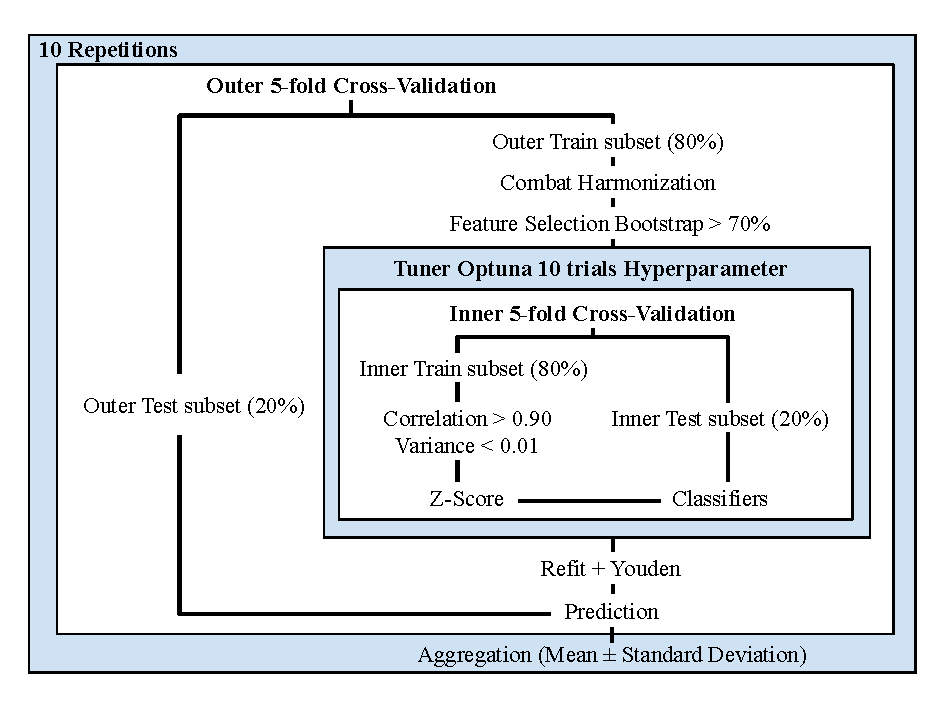
\includegraphics[width=1.0\textwidth]{graphics/nestedcv.pdf}
	\caption{Diagrama da arquitetura de validação cruzada aninhada restrita ao nível do paciente.}
	\label{fig:nestedcv}
\end{figure}

A arquitetura iterativa englobou um ciclo externo composto por 5 partições ($k_{\mathrm{out}}=5$), repetido 10 vezes ($R=10$), totalizando 50 avaliações de generalização independentes por configuração. Para assegurar a reprodutibilidade exata, o gerador pseudoaleatório do ciclo externo adotou a semente determinística $42+1000r$ (sendo $r$ o índice da repetição). O ciclo interno de sintonia (com $k_{\mathrm{in}}=5$) derivou sua respectiva inicialização espacial da fórmula $42+1000r+\mathrm{fold}$.

\textbf{Dinâmica do Ciclo Externo.} Em cada iteração externa, todos os procedimentos supervisionados foram ajustados exclusivamente sobre os pacientes do conjunto de treinamento. O conjunto de atributos retidos por estabilidade (\emph{pool} \code{l1\_stable}) foi construído uma \textbf{única vez} nesta etapa, empregando-se até $B=50$ réplicas \emph{bootstrap} (conforme Eqs.~\eqref{eq:l1-logistic}--\eqref{eq:stability-freq}). O ponto de operação ideal $\tau^*$ (Eq.~\ref{eq:youden}) foi estimado no treinamento externo por meio de predições cruzadas internas (\code{cross\_val\_predict}) e reservado para aplicação estrita no correspondente \emph{fold} de teste.

\textbf{Dinâmica do Ciclo Interno e Seleção.} A sintonia hiperparamétrica do classificador e do \emph{pipeline} a jusante ocorreu no treinamento externo mediante um ciclo interno estratificado, guiado pelo algoritmo Optuna TPE (configurado para 10 ensaios, maximizando a AUC média probabilística interna). O \emph{pipeline} analítico seguiu o fluxo sequencial: filtragem estatística cruzada (\code{CorrVarSelector}: exclusão por correlação $|\rho|>0{,}85$ seguida de variância $<0{,}01$) $\to$ padronização (\code{StandardScaler}) $\to$ Classificação (SVM com \code{probability=True}). Crucialmente, durante o \emph{split} interno, a padronização e a filtragem estatística foram reajustadas sob os dados de treino internos, porém limitadas ao subespaço do \emph{pool} \code{l1\_stable} (o qual não sofreu reconstrução a cada sub-iteração). Como salvaguarda de dimensionalidade, caso os limiares estatísticos internos exaurissem o espaço de atributos, o vetor original selecionado pelo \emph{pool} era restaurado.

\textbf{Agregação e Isolamento Metodológico.} Ao término da busca interna, a configuração hiperparamétrica vencedora foi integralmente reajustada sobre o conjunto completo de treinamento externo, promovendo o recalibrar final dos filtros, do escore Z e da calibração logística de Platt. Ao conjunto de teste externo aplicou-se unicamente as transformações infereciais diretas (\code{transform} e \code{predict\_proba}). Dentro de cada repetição $r$, os cinco \emph{folds} de teste foram concatenados, originando um vetor completo com exatamente uma predição \emph{Out-Of-Fold} (OOF) probabilística por participante. As dez probabilidades resultantes por sujeito foram agregadas por média aritmética antes do cômputo da métrica primária $\mathrm{AUC}_{\mathrm{patient}}$ (Eq.~\ref{eq:auc-pooled}). Reiteramos que este delineamento aninhado encapsulou a totalidade das transformações dependentes da amostra; os domínios pré-processuais da imagem, o controle de qualidade geométrico e a construção paramétrica dos \emph{templates} normativos permaneceram estritamente independentes e foram processados previamente ao engajamento da malha de validação cruzada.

\subsection{Normalização e seleção de atributos}
\label{sec:feature-selection}

\textbf{Tratamento dimensional e normalização.}
Todos os atributos preditivos restringiram-se ao hipocampo bilateral. Na família volumétrica reteve-se apenas as frações teciduais intrarregionais (\code{gm\_norm}, \code{wm\_norm}, \code{csf\_norm}) e o volume de malha \code{original\_shape\_MeshVolume}; os volumes absolutos em mm$^3$ (\code{mask\_mm3}, \code{gm\_mm3}, \ldots) saíram do modelo. As frações teciduais já estão normalizadas à máscara da ROI e \textbf{não} foram divididas pelo ICV. Os descritores de tamanho do PyRadiomics receberam homotetia de ICV: eixos e diâmetros$/\,\mathrm{ICV}^{1/3}$, \code{SurfaceArea}$/\,\mathrm{ICV}^{2/3}$, \code{MeshVolume}$/\,\mathrm{ICV}$, e \code{SurfaceVolumeRatio}$\times\mathrm{ICV}^{1/3}$. Esfericidade, elongação e achatamento são adimensionais e não se alteram. \code{MeshVolume} (já $/\mathrm{ICV}$) entrou na família \emph{vol}, não em \emph{shape}. Esta correção é geométrica (invariância de escala da calote), distinta do \code{StandardScaler} a jusante. Textura GLCM, estatísticas de primeira ordem (sem \code{Energy}/\code{TotalEnergy}) e momentos do campo de deslocamento normativo permaneceram nas unidades originais, sem correcção por ICV.

\textbf{Representação temporal e estruturação multimodal.}
A matriz preditiva é \emph{wide}: um vector por paciente. Em \code{t1\_only} entram só os descritores da visita basal $T_1$. Na representação longitudinal Q4 (\code{t1\_d21\_d32}), cada descritor entra como
\[
\{\mathrm{feat}_{T_1},\,\Delta_{21},\,\Delta_{32}\},
\qquad
\Delta_{21}=\mathrm{feat}_{T_2}-\mathrm{feat}_{T_1},\quad
\Delta_{32}=\mathrm{feat}_{T_3}-\mathrm{feat}_{T_2}.
\]
Não se concatenam os níveis crus de $T_2$ e $T_3$, nem \(\Delta_{31}\). A chave anatómica (\code{anatomical\_key}) suprime o token temporal (\(T_1\), \(D_{21}\), \(D_{32}\)), de modo que p.ex.\ \code{hippocampus\_L\_T1\_gm\_norm} e \code{hippocampus\_L\_D21\_gm\_norm} partilham a raiz \code{hippocampus\_L\_gm\_norm}. Cada família (volume, forma, textura, first-order, deslocamento) foi avaliada de forma unimodal. A multimodalidade reportada é fusão tardia: média dos escores de cinco SVMs, um por família. A concatenação precoce (\emph{early fusion}) de todas as famílias ficou de fora.

\textbf{Selecção por estabilidade \(\ell_1\) (\code{l1\_stable}).}
O filtro ancora-se na frequência empírica de selecção sob penalização \(\ell_1\) com \emph{bootstrap} \citep{bach-2008,meinshausen-2010}, mas \textbf{não} implementa a \emph{stability selection} canónica nem o controlo teórico da PFER. Em cada \emph{fold} externo a selecção corre \textbf{uma vez}, só no treino, e devolve um \emph{pool} de colunas; a SVM nunca vê a classe completa. Cascata no treino externo:

\begin{enumerate}
	\item \textbf{Padronização.} Escore Z (\code{StandardScaler}) com média e desvio só do treino externo.
	\item \textbf{Colinearidade.} Poda gulosa \(|\rho|>0{,}85\). De cada par colinear fica o atributo com maior \(|\rho|\) com \(y\). Pares com a mesma \code{anatomical\_key} (p.ex.\ \(T_1\) e \(\Delta_{32}\) do mesmo descritor) \textbf{não} se eliminam mutuamente.
	\item \textbf{Variância.} Remove colunas com variância \(<0{,}01\) \emph{após} o Z (na prática, quase só constantes). Se o filtro esvaziar o espaço, relaxa para \(\mathrm{var}>0\); não restaura a classe original.
	\item \textbf{Bootstrap \(\times\) L1.} Sobre o subespaço já podado, \(B=50\) amostras com reposição. Réplicas com uma só classe são descartadas. Em cada réplica biclasse volta a aplicar-se um Z \emph{intra-bootstrap} e ajusta-se
	\begin{equation}
		\begin{aligned}
			\hat{\boldsymbol{\beta}}^{(b)},\,\hat{\beta}_0^{(b)}
			&= \arg\min_{\boldsymbol{\beta},\beta_0}
			\left\{
			\sum_{i=1}^{n_{\mathrm{train}}^{(b)}}
			\ell\!\left(y_i,\,\sigma(\mathbf{x}_i^{\top}\boldsymbol{\beta}+\beta_0)\right)
			+ C^{-1}\|\boldsymbol{\beta}\|_1
			\right\}, \\
			\ell(y,p) &= -y\log p-(1-y)\log(1-p),
		\end{aligned}
		\label{eq:l1-logistic}
	\end{equation}
	com solver SAGA, \(C=0{,}1\) fixo. O intercepto \(\beta_0\) não sofre \(\ell_1\). Seja \(\mathcal{M}^{(b)}=\{j:\lvert\hat{\beta}^{(b)}_j\rvert>10^{-9}\}\). Réplicas com \(\mathcal{M}^{(b)}=\emptyset\) não entram no denominador \(B_{\mathrm{eff}}\).
\end{enumerate}

A frequência é por \textbf{grupo} \(g\) (\code{anatomical\_key}), não por coluna:
\begin{equation}
	\pi_g = \frac{1}{B_{\mathrm{eff}}}\sum_{b=1}^{B_{\mathrm{eff}}} \mathbb{I}\!\left(g\cap\mathcal{M}^{(b)}\ne\emptyset\right).
	\label{eq:stability-freq}
\end{equation}
Com \code{stable-pool-min-timepoints=0} e \(\tau=0{,}70\), se \(\pi_g\ge\tau\) o \emph{pool} inclui \textbf{todas} as cronologias desse grupo (\(T_1\), \(D_{21}\), \(D_{32}\)), inclusive as que o corr/var tinham cortado antes do bootstrap.

\textbf{Fallbacks e Optuna.}
Se \(B_{\mathrm{eff}}=0\) ou nenhum grupo atinge \(\tau\), o \emph{pool} reverte primeiro às colunas sobreviventes do corr/var (\code{corr\_fallback}); se ainda vazio, fica a coluna de maior variância no treino \emph{cru} (\code{var\_fallback}). Nunca se restaura a classe completa. O CV interno (Optuna) \textbf{não} repete o bootstrap L1. No espaço já autorizado aplica de novo corr \(|\rho|>0{,}85\) e var \(<0{,}01\) --- aqui \textbf{antes} do scaler, sobre os valores crus do \emph{pool} --- e só depois o Z e o classificador.

\sugestao{}{Continuar}

\subsection{Protocolo de modelagem}
\label{sec:protocolo-oficial}

Protocolo oficial: SVM com \code{probability=True} (Platt), \code{l1\_stable}, nested estratificada $5$ folds $\times$ $10$ repetições (semente $42+1000r$), 50 avaliações externas.
Dobras por identificador de paciente.

\paragraph{Hiperparâmetros.}
Optuna TPE, 10 ensaios, AUC média do CV interno.
SVM: $C\in[10^{-2},10]$ (log), kernel $\in\{\mathrm{linear},\mathrm{RBF}\}$, $\gamma=\mathrm{scale}$, \code{class\_weight} $\in\{\mathrm{None},\mathrm{balanced}\}$, \code{max\_iter}$=2000$.
Um único classificador em todos os contrastes; não se varre RF nem elastic-net.

\paragraph{Youden.}
$\tau^{*}$ maximiza $J=\mathrm{TPR}+\mathrm{TNR}-1$ nas OOF do treino externo e aplica-se só ao teste dessa dobra.
A AUC primária não usa limiar.

\paragraph{AUC no paciente.}
Média de todos os scores OOF do sujeito (fold$\times$repeat); com $5$ testes disjuntos isso é a média das $R=10$ probabilidades.
Uma AUC de Mann--Whitney nos $n$ pares $(y_i,\bar{s}_i)$ (Eqs.~\ref{eq:auc-agg}--\ref{eq:auc-pooled}).
O $\pm$ nas tabelas de ponto é o SD bootstrap dessa AUC paciente ($2000$ reamostragens), \textbf{não} o DP das 50 dobras.

\subsection{Fusão multimodal e preditores clínicos}
\label{sec:fusao}

Fusão tardia (\emph{late fusion}). A multimodalidade oficial não concatena atributos de famílias distintas num único classificador (\emph{early fusion} / \code{--modality all}), o que, em Q4, produziria centenas de colunas com $n$ pequeno e misturaria escalas heterogéneas (fracções volumétricas, GLCM, momentos do DVF) num só rastreio $\ell_1$ \cite{kittler-1998,kuncheva-2004}. Em vez disso, adoptou-se fusão tardia por média de scores: cada família (volume, forma, textura GLCM, primeira ordem, deslocamento) treina a sua própria SVM sob o mesmo protocolo unimodal (CV aninhada ao nível do paciente, l1\_stable, Optuna, \code{combat false}), e as probabilidades OOF por paciente são combinadas \emph{a posteriori} \cite{kittler-1998,dietterich-2000}. Assim, a dimensionalidade efectiva cresce com o número de modelos, não com a união do espaço de atributos; a forma não “vê” 144 colunas GLCM, nem o volume compete com first-order no mesmo pool.

Especificações. Três especificações de slots \code{modalidade:representação} foram pré-definidas (run\_ablation\_full.sh): \begin{itemize} \item tudo em \code{t1\_only}: \code{vol:t1\_only,shape:t1\_only,texture:t1\_only,disp:t1\_only,firstorder:t1\_only}; \item tudo em Q4: as cinco famílias com \code{t1\_d21\_d32}; \item âncora: \code{shape:t1\_only} e as restantes em \code{t1\_d21\_d32} (default de \code{DEFAULT\_LATE\_FUSION\_SPEC}). \end{itemize} Cada especificação corre nas quatro coortes de janela. O identificador de protocolo é um \emph{fingerprint} estável do conjunto de slots (late\_\_\{fp\}); a saída grava-se em \code{ablation\_results\_late\_fusion/\{fingerprint\}/}.

Implementação. O script \code{5\_ablation\_late\_fusion.py} invoca \code{run\_late\_fusion\_ablation\_suite}. Por omissão (\code{--reuse-disk}), cada branch lê o CSV unimodal já gerado (ablation\_results\_* / \{mod\} / ablation\_results\_all.csv), filtrado por tarefa, modelo, ComBat e modo de selecção — as mesmas partições externas (semente 42, 10 repetições × 5 folds) que o mono, para alinhamento fold a fold. Só com \code{--run-missing} se reexecuta a CV aninhada de uma branch ausente. Exigem-se $\geq 2$ branches; a interseção de chaves (task, model, combat, selection, repeat\_id, fold) deve ser não vazia (caso contrário o alinhamento temporal/espacial das partições falhou).

Para cada fold comum, as listas \texttt{test\_id\_pts}, \texttt{test\_y\_true}
e \texttt{test\_scores} de cada branch são expandídas e alinhadas por
\texttt{ID\_PT} (\emph{inner join}): pacientes em falta numa branch saem
desse fold. Sejam $s_{ik}$ a probabilidade OOF
(\texttt{predict\_proba}) do paciente $i$ na branch $k=1,\ldots,K$
e pesos $w_k\geq 0$ com $\sum_k w_k=1$. A configuração primária usa
\code{--combine mean} (pesos uniformes $w_k=1/K$); \code{weighted}
exige \code{--weights} explícitos e não entra no claim. O score fundido é
\begin{equation}
\bar{s}_i = \sum_{k=1}^{K} w_k\, s_{ik}.
\label{eq:late-mean}
\end{equation}
Não há meta-classificador empilhado (\emph{stacking}) nem re-treino sobre
os scores das branches \cite{wolpert-1992}: a fusão é só agregação de
decisões probabilísticas já calibradas por Platt em cada SVM.

Métricas e limiar. AUC, average precision e métricas com limiar recalculam-se sobre ${\bar{s}_i}$ no fold. O limiar binário herdado no CSV late é o threshold da \textbf{primeira} branch da especificação (não se reestima Youden sobre $\bar{s}$); a AUC paciente primária depende só das probabilidades mediadas e não desse limiar. A auditoria selected\_features concatena os atributos escolhidos em todas as branches (soma de cardinalidades em n\_features\_*), para rastreio, sem significar um único espaço concatenado.

Parâmetros do paper (COMMON\_FUSION em run\_ablation\_full.sh): \code{smci\_pmci}, \code{l1\_stable}, SVM, \code{combat false}, 10 repetições, Optuna 10 trials, pool $\pi\geq 70,\%$, $B=50$, $C=0{,}1$, \code{stable-pool-min-timepoints=0}, \code{--combine mean}, \code{--reuse-disk}.

A fusão tardia \textbf{não} retreina um meta-classificador.
Reutiliza os scores OOF \code{predict\_proba} dos cinco SVMs unimodais já ajustados no mesmo nested (mesma semente $\Rightarrow$ mesmos splits).
Por (repetição $r$, dobra $f$), alinhamento inner-join em \code{ID\_PT} e média simples
\begin{equation}
s_{i,r,f}^{\mathrm{late}}
=
\frac{1}{5}\sum_{k=1}^{5} s_{i,r,f}^{(k)}.
\label{eq:late-mean}
\end{equation}
A AUC paciente (Eqs.~\ref{eq:auc-agg}--\ref{eq:auc-pooled}) calcula-se sobre $\{s_{i,r,f}^{\mathrm{late}}\}$ como nas famílias isoladas.
Pesos iguais; sem stacking, sem SVM de segundo nível, sem \code{weighted}.
Cada ramo tem o seu pool \code{l1\_stable}, scaler, Optuna e Platt; forma não vê 144 GLCM e $p\gg n$ da concatenação não se aplica.
Três especificações \textbf{pré-especificadas} (não escolhidas a posteriori):
tudo \code{t1\_only}; tudo Q4; âncora \textbf{forma em \code{t1\_only} $\cup$ volume, textura, deslocamento e primeira ordem em Q4} (cinco ramos, não seis: shape não entra também em Q4).
A AUC primária da fusão não usa limiar.
Sens/Esp da linha late, se reportadas, herdam o $\tau^{*}$ do primeiro ramo da spec (não se reestima Youden no score médio).
A fusão precoce entre famílias de imagem está fora do paper.

Preditores clínicos de $i_0$ (extra, mesmo SVM): sexo, idade, MMSE, ADAS e FAQ (sem CDR global).
A fusão clínica$+$imagem concatena, no treino externo, esses cinco escores $z$-score à forma em \code{t1\_only}; um único SVM.
O protocolo \emph{leaky} (apêndice) estima $z$-score, filtros e pool \code{l1\_stable} no conjunto completo antes da CV.

\subsection{Métrica primária e papéis do bootstrap}
\label{sec:stats}


A métrica oficial é a AUC no paciente $\widehat{\mathrm{AUC}}_{\mathrm{agg}}$ (Eqs.~\ref{eq:auc-agg}--\ref{eq:auc-pooled}), não a média das 50 AUCs de fold nem a AUC \emph{pooled}.
CV aninhada $5\times 10$ no identificador do paciente: em cada repetição $r$ o sujeito $i$ cai uma vez no teste e recebe a probabilidade OOF $s_{ir}$ (\code{predict\_proba}; SVM com Platt).
Primeiro tira-se a média,
\[
\bar{s}_i = \frac{1}{10}\sum_{r=1}^{10} s_{ir},
\]
e calcula-se uma única vez a AUC de Mann--Whitney nos $n$ pares $(y_i,\bar{s}_i)$.
A AUC primária não usa limiar de Youden.

Há \textbf{três} bootstraps, com papéis separados.
Nenhum reexecuta a pipeline nested.
A permutação de rótulos \textbf{não} é bootstrap.

\paragraph{A.~\code{l1\_stable} (dentro da CV).}
Modo \code{l1\_stable}, uma vez por treino externo: $z$-score $\to$ corr $0.85$ $\to$ var $0.01$ $\to$ $B=50$ L1 (Eqs.~\ref{eq:l1-logistic}--\ref{eq:stability-freq}).
Frequência $\pi_g$ por \code{anatomical\_key}; entra o grupo com $\pi_g\ge 70\%$ e \textbf{todos} os seus instantes.
Pool vazio $\to$ \code{corr\_fallback}, nunca a classe inteira.
Esse bootstrap \textbf{não} estima AUC: só escolhe colunas.
Não é o stability selection clássico e não herda PFER~\cite{bach-2008,meinshausen-2010}.
Detalhe: Sec.~\ref{sec:feature-selection}.

\paragraph{B.~Desvio nas tabelas e barras de erro (depois da CV).}
Scores congelados $\{\bar{s}_i\}$.
$B_{\mathrm{sd}}=2000$ reamostragens de pacientes com reposição; em cada uma recalcula-se $\widehat{\mathrm{AUC}}_{\mathrm{agg}}$.
O $\pm$ reportado (Tabelas~\ref{tab:uni_4}--\ref{tab:late_4}) é o desvio-padrão dessas $2000$ AUCs,
\[
\widehat{\sigma}_{\mathrm{boot}}
= \mathrm{sd}\bigl\{\widehat{\mathrm{AUC}}_{\mathrm{agg}}^{(b)}\bigr\}_{b=1}^{B_{\mathrm{sd}}},
\]
\textbf{não} o DP das 50 folds e \textbf{não} um intervalo de confiança a 95\%.

\paragraph{C.~Inferência do $\Delta$AUC (depois da CV).}
Contrastes pareados no mesmo sujeito (p.ex.\ Q4 vs \code{t1\_only}): $B_{\mathrm{boot}}=5000$ reamostragens,
\[
\Delta^{(b)}
= \widehat{\mathrm{AUC}}_{\mathrm{agg}}(A^{(b)})
- \widehat{\mathrm{AUC}}_{\mathrm{agg}}(B^{(b)}).
\]
IC95\% percentílico $[2{,}5,\,97{,}5]$ da distribuição empírica de $\Delta^{(b)}$.
\[
p_{\mathrm{unilateral}}
= \frac{\#\{\Delta^{(b)}\le 0\}+1}{B_{\mathrm{eff}}+1}
\qquad
(\mathrm{H}_1{:}\ \mathrm{AUC}_A>\mathrm{AUC}_B).
\]
$p$ bilateral $=2\min(p_{\mathrm{uni}},1-p_{\mathrm{uni}})$, reservado a contrastes sem direção pré-especificada (imagem vs clínico).
No contraste temporal unimodal, o $q$ é FDR de Benjamini--Hochberg nos cinco $p$ unilaterais da mesma coorte.

\paragraph{Permutação contra o acaso.}
Embaralha-se $y$ com $\{\bar{s}_i\}$ fixos, $B_{\mathrm{perm}}=5000$;
$p=(r+1)/(B_{\mathrm{perm}}+1)$, em que $r$ é o número de permutações com AUC $\ge$ à observada.

$\alpha=0.05$.
O contraste temporal principal é Q4 versus \code{t1\_only} nas cinco famílias, nas quatro coortes.
Pontos das tabelas de resultados são $\widehat{\mathrm{AUC}}_{\mathrm{agg}}$; $p$/$q$ pareados destes CSVs não se herdaram do protocolo \code{t1\_deltas}.

\subsection{Testes estatísticos}
\label{sec:testes}

Todos os contrastes de AUC usam os scores agregados por paciente, não as AUCs de dobra.
\begin{itemize}
\item Permutação de rótulos com scores congelados ($B_{\mathrm{perm}}=5000$): $p=(r+1)/(B+1)$; o pipeline nested \textbf{não} se reexecuta.
\item Bootstrap pareado do $\Delta$AUC ($B_{\mathrm{boot}}=5000$), IC percentílico a 95\%, $p$ unilateral (H$_1$: AUC$_A>$AUC$_B$) e bilateral.
\item FDR de Benjamini--Hochberg sobre os $p$ unilaterais das cinco famílias, dentro de cada coorte.
\item Demografia em \code{36m\_6m}: Mann--Whitney na idade, $\chi^2$ no sexo; classificadores univariados de idade e de sexo com permutação.
\end{itemize}
$\alpha=0.05$.

% =============================================================================
\section{Resultados}\label{sec:Results}

Apresentação: \textbf{uma matriz para as quatro células}, não quatro relatos paralelos.
Protocolo fixo SVM $+$ \code{l1\_stable}.
Métrica: AUC paciente $\widehat{\mathrm{AUC}}_{\mathrm{agg}}$; $\pm$ é SD bootstrap ($B=2000$).
$\Delta=\mathrm{AUC}(\mathrm{Q4})-\mathrm{AUC}(\code{t1\_only})$.
Claim multimodal e nomes de atributos: \code{48m\_12m} ($n=120$); o fatorial testa se o padrão se replica.

\subsection{Demografia}
\label{subsec:demo}

Em \code{36m\_6m} ($n=231$), idade e sexo não diferem entre sMCI e pMCI (Mann--Whitney $p=0.071$; $\chi^2$ $p=0.113$).
Classificador só com idade: AUC $0.560$; só com sexo: $0.452$.
A classificação hipocampal não se reduz a demografia (Tabela~\ref{tab:clin_cohorts}).

\subsection{Uniclasse: Q4 versus \texorpdfstring{\code{t1\_only}}{t1\_only} nas quatro coortes}
\label{subsec:unimodal}

A Tabela~\ref{tab:uni_4} é o resultado principal unimodal.

\begin{sidewaystable}[htbp]
\centering
\footnotesize
\setlength{\tabcolsep}{3.5pt}
\caption{AUC no paciente, SVM.
Em cada célula: \code{t1\_only} / Q4 / $\Delta$.
Negrito: maior das duas representações naquela família$\times$coorte.
$n$: 231, 154, 193, 120.}
\label{tab:uni_4}
\begin{tabular}{@{}l ccc ccc ccc ccc@{}}
\toprule
& \multicolumn{3}{c}{\code{36m\_6m}} & \multicolumn{3}{c}{\code{36m\_12m}} & \multicolumn{3}{c}{\code{48m\_6m}} & \multicolumn{3}{c}{\code{48m\_12m}} \\
\cmidrule(lr){2-4}\cmidrule(lr){5-7}\cmidrule(lr){8-10}\cmidrule(lr){11-13}
Família & $i_0$ & Q4 & $\Delta$ & $i_0$ & Q4 & $\Delta$ & $i_0$ & Q4 & $\Delta$ & $i_0$ & Q4 & $\Delta$ \\
\midrule
vol & 0.738 & \textbf{0.752} & $+0.014$ & \textbf{0.707} & 0.687 & $-0.019$ & 0.714 & \textbf{0.759} & $+0.045$ & 0.632 & \textbf{0.662} & $+0.030$ \\
& $\pm$0.032 & $\pm$0.032 & & $\pm$0.047 & $\pm$0.052 & & $\pm$0.038 & $\pm$0.036 & & $\pm$0.054 & $\pm$0.051 & \\
shape & 0.789 & \textbf{0.795} & $+0.006$ & \textbf{0.739} & 0.732 & $-0.006$ & \textbf{0.801} & 0.797 & $-0.004$ & \textbf{0.761} & 0.755 & $-0.006$ \\
& $\pm$0.030 & $\pm$0.030 & & $\pm$0.046 & $\pm$0.047 & & $\pm$0.035 & $\pm$0.035 & & $\pm$0.043 & $\pm$0.043 & \\
texture & 0.727 & \textbf{0.739} & $+0.012$ & 0.724 & \textbf{0.745} & $+0.021$ & 0.740 & \textbf{0.759} & $+0.019$ & 0.711 & \textbf{0.762} & $+0.052$ \\
& $\pm$0.034 & $\pm$0.033 & & $\pm$0.051 & $\pm$0.051 & & $\pm$0.037 & $\pm$0.036 & & $\pm$0.050 & $\pm$0.044 & \\
firstorder & 0.752 & \textbf{0.768} & $+0.016$ & 0.741 & \textbf{0.760} & $+0.020$ & 0.773 & \textbf{0.797} & $+0.024$ & 0.719 & \textbf{0.737} & $+0.019$ \\
& $\pm$0.032 & $\pm$0.031 & & $\pm$0.051 & $\pm$0.050 & & $\pm$0.035 & $\pm$0.033 & & $\pm$0.048 & $\pm$0.048 & \\
disp & \textbf{0.628} & 0.501 & $-0.127$ & 0.476 & \textbf{0.492} & $+0.016$ & \textbf{0.609} & 0.571 & $-0.038$ & 0.524 & \textbf{0.621} & $+0.097$ \\
& $\pm$0.036 & $\pm$0.039 & & $\pm$0.057 & $\pm$0.056 & & $\pm$0.043 & $\pm$0.043 & & $\pm$0.055 & $\pm$0.052 & \\
\bottomrule
\end{tabular}
\end{sidewaystable}

\paragraph{Leitura da matriz.}
\begin{itemize}
\item \textbf{Textura e primeira ordem:} $\Delta>0$ nas quatro células. Máximo de textura $+0.052$ em \code{48m\_12m} ($0.711\to 0.762$).
\item \textbf{Volume:} $\Delta>0$ em três células; quebra em \code{36m\_12m} ($-0.019$).
\item \textbf{Forma:} teto estático. Q4 nunca ganha de forma material ($|\Delta|\le 0.006$). Melhor unimodal em \code{36m\_6m}/\code{48m\_6m}/\code{48m\_12m} é shape-$i_0$ (ou empate com textura Q4 no claim: $0.762$ vs $0.761$).
\item \textbf{Deslocamento:} fraco. Em intervalos de 12 meses o pool \code{l1\_stable} esvazia-se na maioria das dobras (\code{corr\_fallback}); o $\Delta$ positivo em \code{48m\_12m} \textbf{não} se interpreta como selecção estável.
\end{itemize}
Q4 agrega nas famílias de intensidade/volume e \textbf{não} passa o teto shape-$i_0$ de forma consistente.

\subsection{Quantos e quais atributos}
\label{subsec:atributos-sel}

A Tabela~\ref{tab:nfeat} é a média de colunas que o SVM vê após \code{l1\_stable} ($50$ avaliações).
A Tabela~\ref{tab:feat_claim} lista os grupos com cobertura $\ge 20\%$ em \code{48m\_12m}.

\begin{table}[htbp]
\centering
\footnotesize
\caption{Média de atributos seleccionados (min--máx nas 50 dobras).
Entra: Tabela~\ref{tab:dims}.
Disp em 12\,meses: maioria \code{corr\_fallback}.}
\label{tab:nfeat}
\begin{tabular}{ll rr rr rr rr}
\toprule
& & \multicolumn{2}{c}{\code{36m\_6m}} & \multicolumn{2}{c}{\code{36m\_12m}} & \multicolumn{2}{c}{\code{48m\_6m}} & \multicolumn{2}{c}{\code{48m\_12m}} \\
\cmidrule(lr){3-4}\cmidrule(lr){5-6}\cmidrule(lr){7-8}\cmidrule(lr){9-10}
Fam. & enc & média & faixa & média & faixa & média & faixa & média & faixa \\
\midrule
vol & $i_0$ & 1.00 & 1--1 & 1.18 & 1--4 & 1.08 & 1--2 & 2.14 & 1--5 \\
vol & Q4 & 6.28 & 5--11 & 4.98 & 3--12 & 6.14 & 3--9 & 5.16 & 3--13 \\
shape & $i_0$ & 1.64 & 1--2 & 1.76 & 1--12 & 2.00 & 1--3 & 1.52 & 1--3 \\
shape & Q4 & 7.80 & 3--12 & 4.08 & 3--27 & 7.14 & 6--12 & 5.12 & 3--9 \\
texture & $i_0$ & 1.66 & 1--4 & 2.22 & 1--8 & 1.52 & 1--3 & 1.62 & 1--10 \\
texture & Q4 & 5.38 & 3--15 & 3.74 & 3--25 & 5.32 & 3--12 & 3.60 & 3--6 \\
firstorder & $i_0$ & 3.00 & 1--4 & 1.62 & 1--7 & 2.84 & 2--4 & 1.00 & 1--1 \\
firstorder & Q4 & 10.86 & 4--15 & 3.82 & 3--29 & 9.92 & 6--15 & 3.00 & 3--3 \\
disp & $i_0$ & 1.50 & 1--2 & 13.90 & 1--18 & 1.42 & 1--2 & 15.74 & 1--18 \\
disp & Q4 & 4.92 & 1--10 & 33.08 & 1--50 & 3.72 & 1--9 & 41.62 & 1--50 \\
\bottomrule
\end{tabular}
\end{table}

\begin{table}[htbp]
\centering
\footnotesize
\caption{Grupos retidos em $\ge 20\%$ das 50 avaliações, \code{48m\_12m}.
Cobertura = fracção de folds com o biomarcador (qualquer visita).
Em Q4, T1/D21/D32 do mesmo \code{anatomical\_key} tendem a entrar juntos.}
\label{tab:feat_claim}
\begin{tabular}{lllrr}
\toprule
Família & enc & Grupo & cob.\ (\%) & notas temporais \\
\midrule
vol & $i_0$ & R \code{csf\_norm} & 84 & T1 \\
vol & $i_0$ & L \code{csf\_norm} & 50 & T1 \\
vol & Q4 & L \code{csf\_norm} & 84 & T1$=$D21$=$D32 \\
vol & Q4 & R \code{csf\_norm} & 68 & T1$=$D21$=$D32 \\
shape & $i_0$ & L SurfaceVolumeRatio & 68 & T1 \\
shape & $i_0$ & R SurfaceVolumeRatio & 64 & T1 \\
shape & Q4 & R SurfaceVolumeRatio & 82 & $\approx$ três visitas \\
shape & Q4 & L SurfaceVolumeRatio & 78 & $\approx$ três visitas \\
texture & $i_0$ & L InverseVariance & 62 & T1 \\
texture & Q4 & L InverseVariance & 52 & T1$=$D21$=$D32 \\
firstorder & $i_0$/Q4 & L Entropy / Uniformity & 42 / 38 & Q4: três visitas \\
disp & $i_0$/Q4 & momentos \code{mag}/\code{logjac}/\code{strain\_fro} & $\sim$84--92 & \code{corr\_fallback} \\
\bottomrule
\end{tabular}
\end{table}

L1 corta a classe a poucas colunas (tipicamente 1--6), excepto deslocamento em 12\,meses.
Nomes = frequência, não assinatura única: SurfaceVolumeRatio e \code{csf\_norm} são estáveis; InverseVariance e Entropy/Uniformity são os representantes de textura e primeira ordem.

\subsection{Multimodal: fusão tardia nas quatro coortes}
\label{subsec:multimodal}

A Tabela~\ref{tab:late_4} compara as três especificações ao teto unimodal da mesma célula (máximo da Tabela~\ref{tab:uni_4}).

\begin{table}[htbp]
\centering
\caption{AUC paciente da fusão tardia (média de cinco SVMs) versus teto unimodal.
Âncora: shape@$i_0$ $\cup$ vol/texture/disp/firstorder em Q4.}
\label{tab:late_4}
\begin{tabular}{lrrrr}
\toprule
Coorte & Teto uni. & Late $i_0$ & Late Q4 & Âncora \\
\midrule
\code{36m\_6m} & 0.795 & $0.808\pm 0.029$ & $0.814\pm 0.028$ & $0.814\pm 0.029$ \\
\code{36m\_12m} & 0.760 & $0.769\pm 0.045$ & $0.793\pm 0.039$ & $0.792\pm 0.041$ \\
\code{48m\_6m} & 0.801 & $0.816\pm 0.035$ & $0.828\pm 0.032$ & $\mathbf{0.833\pm 0.032}$ \\
\code{48m\_12m} & 0.762 & $0.761\pm 0.044$ & $\mathbf{0.802\pm 0.040}$ & $\mathbf{0.802\pm 0.040}$ \\
\bottomrule
\end{tabular}
\end{table}

Late Q4 e âncora superam o teto unimodal nas quatro células.
No claim, late $i_0$ \textbf{não} passa o teto ($0.761$ vs shape-$i_0$ $0.761$); quem passa é a união \emph{com} Q4 ($0.802$).
Âncora $\approx$ late Q4: a forma já saturava no baseline; o ganho é empilhar os papéis que se movem no tempo.

\subsection{Clínico, sanidade e literatura}
\label{subsec:controlos}

Em \code{48m\_12m}, SVM só com sexo, idade, MMSE, ADAS e FAQ em $i_0$: $0.812\pm 0.040$.
Fusão precoce clínica$+$forma \code{t1\_only}: $0.843\pm 0.036$.
A RM hipocampal isolada não supera o clínico; acrescentá-la sobe o ponto sem ser o claim das perguntas 1--3.

CN versus AD no mesmo stack (volume Q4, \code{48m\_12m}): $0.833\pm 0.030$ --- a tarefa fácil funciona; sMCI/pMCI permanece a difícil.
Leaky (volume Q4, selecção global): $0.660$ versus nested $0.662$.

A Tabela~\ref{tab:literature_comparison} situa o teto unimodal e a fusão tardia face a estudos sMCI/pMCI representativos.
Os números \textbf{não} são comparáveis: diferem horizonte, ROI, preditores clínicos e validação.

\begin{sidewaystable}[htbp]
\centering
\footnotesize
\setlength{\tabcolsep}{4pt}
\renewcommand{\arraystretch}{1.15}
\caption{Comparação indicativa de desempenho prognóstico publicado em sMCI versus pMCI e dos resultados ADNI deste estudo sob validação aninhada no paciente.}
\label{tab:literature_comparison}
\begin{tabular}{@{}lllccc@{}}
\toprule
\textbf{Estudo} & \textbf{Base} & \textbf{Atributos} &
\textbf{Validação} & \textbf{AUC} & \textbf{Sens / Esp (\%)} \\
\midrule
\citet{bucholc-2023} & NACC &
Cognitivo + funcional &
3 visitas; CV retido &
$0.601 \pm 0.054$ & $95.4 \pm 1.8$ / $24.7 \pm 12.0$ \\
\citet{bucholc-2023} & NACC &
Cognitivo + funcional &
4 visitas; CV retido &
$0.756 \pm 0.103$ & $92.9 \pm 4.6$ / $58.3 \pm 19.1$ \\
\citet{grassi-2019} & ADNI &
Sociodemográfico + clínico &
Baseline; CV 10 folds &
$0.88$ & $77.7$ / $79.9$ \\
\citet{moradi-2015} & ADNI &
Densidade de GM (cérebro inteiro) &
Baseline; CV 10 folds &
$0.766$ & $88.9$ / $51.6$ \\
\citet{moradi-2015} & ADNI &
GM (cérebro inteiro) + cognitivo &
Baseline; CV 10 folds &
$0.902$ & $86.7$ / $73.6$ \\
\citet{ye-2012}$^{\S}$ & ADNI &
Cérebro inteiro + cognitivo &
Baseline; stability selection &
$0.859$ & \textemdash\ / \textemdash \\
\citet{casanova-2013}$^{\P}$ & ADNI &
Tecidos (cérebro inteiro) + cognitivo &
Baseline; CV aninhada &
\textemdash & $45.8$ / $75.5$ \\
\citet{guo-2017a}$^{\|}$ & ADNI &
Córtex &
Baseline; LOOCV &
\textemdash & $85.0$ / $84.8$ \\
\citet{cuingnet-2011} & ADNI &
Volume hipocampal &
Baseline; LOOCV &
\textemdash & $62.0$ / $69.0$ \\
\midrule
\textbf{Este trabalho (teto $i_0$)}$^{\dagger}$ & ADNI &
Forma hipocampal &
$i_0$; nested CV (SVM) &
$\mathbf{0.761 \pm 0.043}$ & $\mathbf{70.5 \pm 15.4}$ / $\mathbf{63.7 \pm 12.7}$ \\
\textbf{Este trabalho (Q4 unimodal)} & ADNI &
Textura GLCM (níveis T1+D21+D32) &
3 visitas; nested CV &
$\mathbf{0.762 \pm 0.044}$ & $\mathbf{68.3 \pm 17.8}$ / $\mathbf{67.3 \pm 15.1}$ \\
\textbf{Este trabalho (fusão tardia)}$^{\ddagger}$ & ADNI &
Âncora / late Q4 (5 SVMs) &
3 visitas; nested CV &
$\mathbf{0.802 \pm 0.040}$ & $\mathbf{74.2 \pm 18.3}$ / $\mathbf{66.8 \pm 14.8}$ \\
\textbf{Este trabalho} & ADNI &
Clínico (sexo, idade, MMSE, ADAS, FAQ) &
$i_0$; nested CV (SVM) &
$\mathbf{0.812 \pm 0.040}$ & $\mathbf{70.0 \pm 14.2}$ / $\mathbf{70.9 \pm 14.1}$ \\
\textbf{Este trabalho} & ADNI &
Clínico $+$ forma $i_0$ &
nested CV (SVM) &
$\mathbf{0.843 \pm 0.036}$ & $\mathbf{77.1 \pm 13.0}$ / $\mathbf{73.2 \pm 13.6}$ \\
\bottomrule
\end{tabular}
\vspace{0.5em}
\begin{flushleft}
\scriptsize
\textit{Nota:}
Linhas próprias: coorte \code{48m\_12m} ($n=120$).
$^{\dagger}$Teto unimodal de baseline (forma, \code{t1\_only}).
$^{\ddagger}$Fusão tardia; Sens/Esp da linha late Q4 (Youden por dobra).
Antes de $\pm$ na AUC: estimando paciente; depois: SD bootstrap ($2000$).
Sens/Esp: média $\pm$ SD nas 50 avaliações externas.
\end{flushleft}
\end{sidewaystable}

\section{Discussão}\label{sec:Discussions}

A pergunta era se níveis longitudinais hipocampais agregam discriminação sMCI/pMCI além do $i_0$.
A resposta depende do \emph{papel} da família e de uniclasse versus união.

\paragraph{Uniclasse agrega, não passa o teto.}
Q4 sobe volume, textura e primeira ordem; a forma já discrimina no $i_0$ e Q4 é redundante (o filtro de correlação nem deixa T1 competir com D21/D32 do mesmo descritor como se fossem mecanismos distintos).
Nenhuma família Q4 substitui de forma consistente o teto shape-$i_0$.

\paragraph{União tardia passa o teto.}
Cinco SVMs, média de scores: forma não vê 144 GLCM; volume não vê firstorder.
Late Q4 e a âncora superam o máximo unimodal nas quatro células.
No claim, late só-$i_0$ empata o teto; o ganho exige os braços Q4.
A âncora é o desenho que o unimodal pede: geometria no baseline, o resto no tempo.

\paragraph{Fatorial, não crowning.}
As quatro coortes não são réplicas independentes, mas o padrão (shape-$i_0$ teto; Q4 em texture/FO/vol; late $>$ teto) sobrevive a janela e intervalo.
Não se coroa \code{wide}, deltas nem early fusion.

\paragraph{Atributos.}
\code{l1\_stable} reduz a classe a poucos representantes (SurfaceVolumeRatio, \code{csf\_norm}, InverseVariance, Entropy/Uniformity).
Frequência across folds, não biomarcador único.
Deslocamento em 12\,meses cai em \code{corr\_fallback}: DVF normativo continua um negativo útil, não um claim.

\paragraph{Clínico.}
Escores de $i_0$ ($0.812$) permanecem competitivos face à imagem hipocampal isolada, alinhado com~\citet{grassi-2019,moradi-2015}.
A RM entra como adjunto; o claim das perguntas 1--3 é interno à imagem.


\section{Conclusões}\label{sec:Conclusions}

Sob validação aninhada no paciente, Q4 (\code{t1\_d21\_d32}) \textbf{agrega} discriminação unimodal em volume, textura e primeira ordem, mas \textbf{não} supera o teto da forma em $i_0$.
A união tardia das cinco famílias --- em especial a âncora forma@$i_0$ $\cup$ restante Q4 --- \textbf{supera} esse teto nas quatro células do fatorial ($0.76\to 0.80$ em \code{48m\_12m}).
\code{l1\_stable} retém poucos representantes estáveis, não uma assinatura única.
Escores clínicos de $i_0$ permanecem competitivos; a RM hipocampal é adjunto estrutural.
O contributo é o protocolo auditável e esta leitura por papéis, não um classificador novo.

\sugestao{}{Limitações} 

\begin{itemize}
	\item \textbf{Uma fonte, caso completo.} Só a ADNI fornece $n$ viável com três RM e rótulo sMCI/pMCI nas janelas 36/48 meses.
	\item \textbf{Soft pMCI.} 46 (intervalos de 6 meses) e 33 (12 meses) têm $i_3$ igual ao primeiro AD.
	\item \textbf{Sobreposição e $n$.} Coortes não independentes; \code{48m\_12m} tem 120 sujeitos.
	\item \textbf{Q4 são níveis, não taxas.} Não se modela $i_b-T_a$.
	\item \textbf{Fallback L1.} Disp em 12\,meses não é pool $\pi\ge 70\%$.
	\item \textbf{Inferência pareada.} Os $p$/$q$ destes CSVs ainda não substituem a tabela FDR do protocolo \code{t1\_deltas}; os pontos e o $\Delta$ são o resultado reportado.
	\item \textbf{ROI única.} Hipocampo de propósito.
	\item \textbf{Operações pré-CV.} QC do MRQy e templates CN estimam-se uma vez no conjunto.
\end{itemize}

\section*{Agradecimentos}

A recolha e a partilha dos dados foram financiadas pela Alzheimer's Disease Neuroimaging Initiative (ADNI).

\subsection*{Financiamento}

O presente trabalho foi realizado com apoio da Coordenação de Aperfeiçoamento de Pessoal de Nível Superior -- Brasil (CAPES) -- Código de Financiamento 001.

\section*{Conflito de interesses}

Os autores declaram não haver conflito de interesses.

\bibliographystyle{cas-model2-names-short}
\biboptions{authoryear}
\bibliography{referencias}
\end{document}
